\documentclass[twoside]{book}

% Packages required by doxygen
\usepackage{fixltx2e}
\usepackage{calc}
\usepackage{doxygen}
\usepackage[export]{adjustbox} % also loads graphicx
\usepackage{graphicx}
\usepackage[utf8]{inputenc}
\usepackage{makeidx}
\usepackage{multicol}
\usepackage{multirow}
\PassOptionsToPackage{warn}{textcomp}
\usepackage{textcomp}
\usepackage[nointegrals]{wasysym}
\usepackage[table]{xcolor}

% Font selection
\usepackage[T1]{fontenc}
\usepackage[scaled=.90]{helvet}
\usepackage{courier}
\usepackage{amssymb}
\usepackage{sectsty}
\renewcommand{\familydefault}{\sfdefault}
\allsectionsfont{%
  \fontseries{bc}\selectfont%
  \color{darkgray}%
}
\renewcommand{\DoxyLabelFont}{%
  \fontseries{bc}\selectfont%
  \color{darkgray}%
}
\newcommand{\+}{\discretionary{\mbox{\scriptsize$\hookleftarrow$}}{}{}}

% Page & text layout
\usepackage{geometry}
\geometry{%
  a4paper,%
  top=2.5cm,%
  bottom=2.5cm,%
  left=2.5cm,%
  right=2.5cm%
}
\tolerance=750
\hfuzz=15pt
\hbadness=750
\setlength{\emergencystretch}{15pt}
\setlength{\parindent}{0cm}
\setlength{\parskip}{3ex plus 2ex minus 2ex}
\makeatletter
\renewcommand{\paragraph}{%
  \@startsection{paragraph}{4}{0ex}{-1.0ex}{1.0ex}{%
    \normalfont\normalsize\bfseries\SS@parafont%
  }%
}
\renewcommand{\subparagraph}{%
  \@startsection{subparagraph}{5}{0ex}{-1.0ex}{1.0ex}{%
    \normalfont\normalsize\bfseries\SS@subparafont%
  }%
}
\makeatother

% Headers & footers
\usepackage{fancyhdr}
\pagestyle{fancyplain}
\fancyhead[LE]{\fancyplain{}{\bfseries\thepage}}
\fancyhead[CE]{\fancyplain{}{}}
\fancyhead[RE]{\fancyplain{}{\bfseries\leftmark}}
\fancyhead[LO]{\fancyplain{}{\bfseries\rightmark}}
\fancyhead[CO]{\fancyplain{}{}}
\fancyhead[RO]{\fancyplain{}{\bfseries\thepage}}
\fancyfoot[LE]{\fancyplain{}{}}
\fancyfoot[CE]{\fancyplain{}{}}
\fancyfoot[RE]{\fancyplain{}{\bfseries\scriptsize Generated by Doxygen }}
\fancyfoot[LO]{\fancyplain{}{\bfseries\scriptsize Generated by Doxygen }}
\fancyfoot[CO]{\fancyplain{}{}}
\fancyfoot[RO]{\fancyplain{}{}}
\renewcommand{\footrulewidth}{0.4pt}
\renewcommand{\chaptermark}[1]{%
  \markboth{#1}{}%
}
\renewcommand{\sectionmark}[1]{%
  \markright{\thesection\ #1}%
}

% Indices & bibliography
\usepackage{natbib}
\usepackage[titles]{tocloft}
\setcounter{tocdepth}{3}
\setcounter{secnumdepth}{5}
\makeindex

% Custom commands
\newcommand{\clearemptydoublepage}{%
  \newpage{\pagestyle{empty}\cleardoublepage}%
}

\usepackage{caption}
\captionsetup{labelsep=space,justification=centering,font={bf},singlelinecheck=off,skip=4pt,position=top}

%===== C O N T E N T S =====

\begin{document}

% Titlepage & ToC
\pagenumbering{alph}
\begin{titlepage}
\vspace*{7cm}
\begin{center}%
{\Large T\+P1\+\_\+\+G\+Collante\+\_\+39022782 }\\
\vspace*{1cm}
{\large Generated by Doxygen 1.8.13}\\
\end{center}
\end{titlepage}
\clearemptydoublepage
\pagenumbering{roman}
\tableofcontents
\clearemptydoublepage
\pagenumbering{arabic}

%--- Begin generated contents ---
\chapter{T\+P1\+: I\+PC -\/ Sockets U\+N\+IX}
\label{md__r_e_a_d_m_e}
Repository for project n°1 \char`\"{}\+I\+P\+C -\/ U\+N\+I\+X Sockets\char`\"{} of the Operative Systems II course of the Computer Engineering degree (F\+C\+E\+FyN, U\+NC). 
\chapter{Data Structure Index}
\section{Data Structures}
Here are the data structures with brief descriptions\+:\begin{DoxyCompactList}
\item\contentsline{section}{\textbf{ msgbuf} }{\pageref{structmsgbuf}}{}
\item\contentsline{section}{\textbf{ my\+\_\+msgbuf} }{\pageref{structmy__msgbuf}}{}
\item\contentsline{section}{\textbf{ user} }{\pageref{structuser}}{}
\end{DoxyCompactList}

\chapter{File Index}
\section{File List}
Here is a list of all files with brief descriptions\+:\begin{DoxyCompactList}
\item\contentsline{section}{cliente/\textbf{ client.\+c} }{\pageref{client_8c}}{}
\item\contentsline{section}{cliente/\textbf{ mbr.\+c} }{\pageref{cliente_2mbr_8c}}{}
\item\contentsline{section}{cliente/\textbf{ prompt.\+c} }{\pageref{prompt_8c}}{}
\item\contentsline{section}{cliente/\textbf{ socket\+\_\+client.\+c} }{\pageref{socket__client_8c}}{}
\item\contentsline{section}{include/\textbf{ auth.\+h} }{\pageref{auth_8h}}{}
\item\contentsline{section}{include/\textbf{ client.\+h} }{\pageref{client_8h}}{}
\item\contentsline{section}{include/\textbf{ common.\+h} }{\pageref{common_8h}}{}
\item\contentsline{section}{include/\textbf{ fileserv.\+h} }{\pageref{fileserv_8h}}{}
\item\contentsline{section}{include/\textbf{ mbr.\+h} }{\pageref{include_2mbr_8h}}{}
\item\contentsline{section}{include/\textbf{ md5.\+h} }{\pageref{md5_8h}}{}
\item\contentsline{section}{include/\textbf{ mq.\+h} }{\pageref{mq_8h}}{}
\item\contentsline{section}{include/\textbf{ prompt.\+h} }{\pageref{prompt_8h}}{}
\item\contentsline{section}{include/\textbf{ server.\+h} }{\pageref{server_8h}}{}
\item\contentsline{section}{include/\textbf{ socket.\+h} }{\pageref{include_2socket_8h}}{}
\item\contentsline{section}{server/\textbf{ auth.\+c} }{\pageref{auth_8c}}{}
\item\contentsline{section}{server/\textbf{ fileserv.\+c} }{\pageref{fileserv_8c}}{}
\item\contentsline{section}{server/\textbf{ md5.\+c} }{\pageref{md5_8c}}{}
\item\contentsline{section}{server/\textbf{ mq.\+c} }{\pageref{mq_8c}}{}
\item\contentsline{section}{server/\textbf{ server.\+c} }{\pageref{server_8c}}{}
\item\contentsline{section}{server/\textbf{ socket\+\_\+server.\+c} }{\pageref{socket__server_8c}}{}
\item\contentsline{section}{thrash/\textbf{ burn.\+c} }{\pageref{burn_8c}}{}
\item\contentsline{section}{thrash/\textbf{ cuarentena.\+c} }{\pageref{cuarentena_8c}}{}
\item\contentsline{section}{thrash/\textbf{ example.\+c} }{\pageref{example_8c}}{}
\item\contentsline{section}{thrash/\textbf{ file.\+c} }{\pageref{file_8c}}{}
\item\contentsline{section}{thrash/\textbf{ fseek.\+c} }{\pageref{fseek_8c}}{}
\item\contentsline{section}{thrash/\textbf{ main.\+c} }{\pageref{main_8c}}{}
\item\contentsline{section}{thrash/\textbf{ mbr.\+c} }{\pageref{thrash_2mbr_8c}}{}
\item\contentsline{section}{thrash/\textbf{ mbr.\+h} }{\pageref{thrash_2mbr_8h}}{}
\item\contentsline{section}{thrash/\textbf{ prueba.\+c} }{\pageref{prueba_8c}}{}
\item\contentsline{section}{thrash/\textbf{ receiver2.\+c} }{\pageref{receiver2_8c}}{}
\item\contentsline{section}{thrash/\textbf{ recfile.\+c} }{\pageref{recfile_8c}}{}
\item\contentsline{section}{thrash/\textbf{ reverse.\+c} }{\pageref{reverse_8c}}{}
\item\contentsline{section}{thrash/\textbf{ sender2.\+c} }{\pageref{sender2_8c}}{}
\item\contentsline{section}{thrash/\textbf{ sendfile.\+c} }{\pageref{sendfile_8c}}{}
\item\contentsline{section}{thrash/\textbf{ signal.\+c} }{\pageref{signal_8c}}{}
\item\contentsline{section}{thrash/\textbf{ socket.\+c} }{\pageref{socket_8c}}{}
\item\contentsline{section}{thrash/\textbf{ socket.\+h} }{\pageref{thrash_2socket_8h}}{}
\item\contentsline{section}{thrash/\textbf{ test.\+c} }{\pageref{test_8c}}{}
\end{DoxyCompactList}

\chapter{Data Structure Documentation}
\section{msgbuf Struct Reference}
\label{structmsgbuf}\index{msgbuf@{msgbuf}}
\subsection*{Data Fields}
\begin{DoxyCompactItemize}
\item 
long \textbf{ mtype}
\item 
char \textbf{ mtext} [1]
\end{DoxyCompactItemize}


\subsection{Field Documentation}
\mbox{\label{structmsgbuf_a25caee4909ab47dffbf18c639cb7f833}} 
\index{msgbuf@{msgbuf}!mtext@{mtext}}
\index{mtext@{mtext}!msgbuf@{msgbuf}}
\subsubsection{mtext}
{\footnotesize\ttfamily char mtext[1]}

\mbox{\label{structmsgbuf_a6e71692f0e74d6cd516fa62386afcfb4}} 
\index{msgbuf@{msgbuf}!mtype@{mtype}}
\index{mtype@{mtype}!msgbuf@{msgbuf}}
\subsubsection{mtype}
{\footnotesize\ttfamily long mtype}



The documentation for this struct was generated from the following file\+:\begin{DoxyCompactItemize}
\item 
\textbf{ test.\+c}\end{DoxyCompactItemize}

\section{my\+\_\+msgbuf Struct Reference}
\label{structmy__msgbuf}\index{my\+\_\+msgbuf@{my\+\_\+msgbuf}}


{\ttfamily \#include $<$mq.\+h$>$}

\subsection*{Data Fields}
\begin{DoxyCompactItemize}
\item 
long \textbf{ mtype}
\item 
char \textbf{ mtext} [\textbf{ B\+U\+F\+F\+S\+I\+ZE}]
\end{DoxyCompactItemize}


\subsection{Field Documentation}
\mbox{\label{structmy__msgbuf_a08fee1c15ded91acf2b246258fce5d9b}} 
\index{my\+\_\+msgbuf@{my\+\_\+msgbuf}!mtext@{mtext}}
\index{mtext@{mtext}!my\+\_\+msgbuf@{my\+\_\+msgbuf}}
\subsubsection{mtext}
{\footnotesize\ttfamily char mtext[\textbf{ B\+U\+F\+F\+S\+I\+ZE}]}

\mbox{\label{structmy__msgbuf_a6e71692f0e74d6cd516fa62386afcfb4}} 
\index{my\+\_\+msgbuf@{my\+\_\+msgbuf}!mtype@{mtype}}
\index{mtype@{mtype}!my\+\_\+msgbuf@{my\+\_\+msgbuf}}
\subsubsection{mtype}
{\footnotesize\ttfamily long mtype}



The documentation for this struct was generated from the following file\+:\begin{DoxyCompactItemize}
\item 
include/\textbf{ mq.\+h}\end{DoxyCompactItemize}

\section{user Struct Reference}
\label{structuser}\index{user@{user}}


{\ttfamily \#include $<$auth.\+h$>$}

\subsection*{Data Fields}
\begin{DoxyCompactItemize}
\item 
char \textbf{ username} [\textbf{ B\+U\+F\+F\+S\+I\+ZE}]
\item 
char \textbf{ password} [\textbf{ B\+U\+F\+F\+S\+I\+ZE}]
\item 
char \textbf{ lastconnect} [\textbf{ B\+U\+F\+F\+S\+I\+ZE}]
\item 
char \textbf{ block} [\textbf{ B\+U\+F\+F\+S\+I\+ZE}]
\end{DoxyCompactItemize}


\subsection{Field Documentation}
\mbox{\label{structuser_a009391444dc8bb1bde591d0d61b68de3}} 
\index{user@{user}!block@{block}}
\index{block@{block}!user@{user}}
\subsubsection{block}
{\footnotesize\ttfamily char block[\textbf{ B\+U\+F\+F\+S\+I\+ZE}]}

\mbox{\label{structuser_af048c958a95d92e5a41ced7657385065}} 
\index{user@{user}!lastconnect@{lastconnect}}
\index{lastconnect@{lastconnect}!user@{user}}
\subsubsection{lastconnect}
{\footnotesize\ttfamily char lastconnect[\textbf{ B\+U\+F\+F\+S\+I\+ZE}]}

\mbox{\label{structuser_aca6a393b357d3af054dc060262ab427e}} 
\index{user@{user}!password@{password}}
\index{password@{password}!user@{user}}
\subsubsection{password}
{\footnotesize\ttfamily char password[\textbf{ B\+U\+F\+F\+S\+I\+ZE}]}

\mbox{\label{structuser_a0a3e67b9f144f2f261876a12d350395b}} 
\index{user@{user}!username@{username}}
\index{username@{username}!user@{user}}
\subsubsection{username}
{\footnotesize\ttfamily char username[\textbf{ B\+U\+F\+F\+S\+I\+ZE}]}



The documentation for this struct was generated from the following file\+:\begin{DoxyCompactItemize}
\item 
include/\textbf{ auth.\+h}\end{DoxyCompactItemize}

\chapter{File Documentation}
\section{cliente/client.c File Reference}
\label{client_8c}\index{cliente/client.\+c@{cliente/client.\+c}}
{\ttfamily \#include \char`\"{}socket.\+h\char`\"{}}\newline
{\ttfamily \#include \char`\"{}prompt.\+h\char`\"{}}\newline
{\ttfamily \#include \char`\"{}common.\+h\char`\"{}}\newline
{\ttfamily \#include $<$termios.\+h$>$}\newline
{\ttfamily \#include $<$errno.\+h$>$}\newline
{\ttfamily \#include $<$unistd.\+h$>$}\newline
Include dependency graph for client.\+c\+:\nopagebreak
\begin{figure}[H]
\begin{center}
\leavevmode
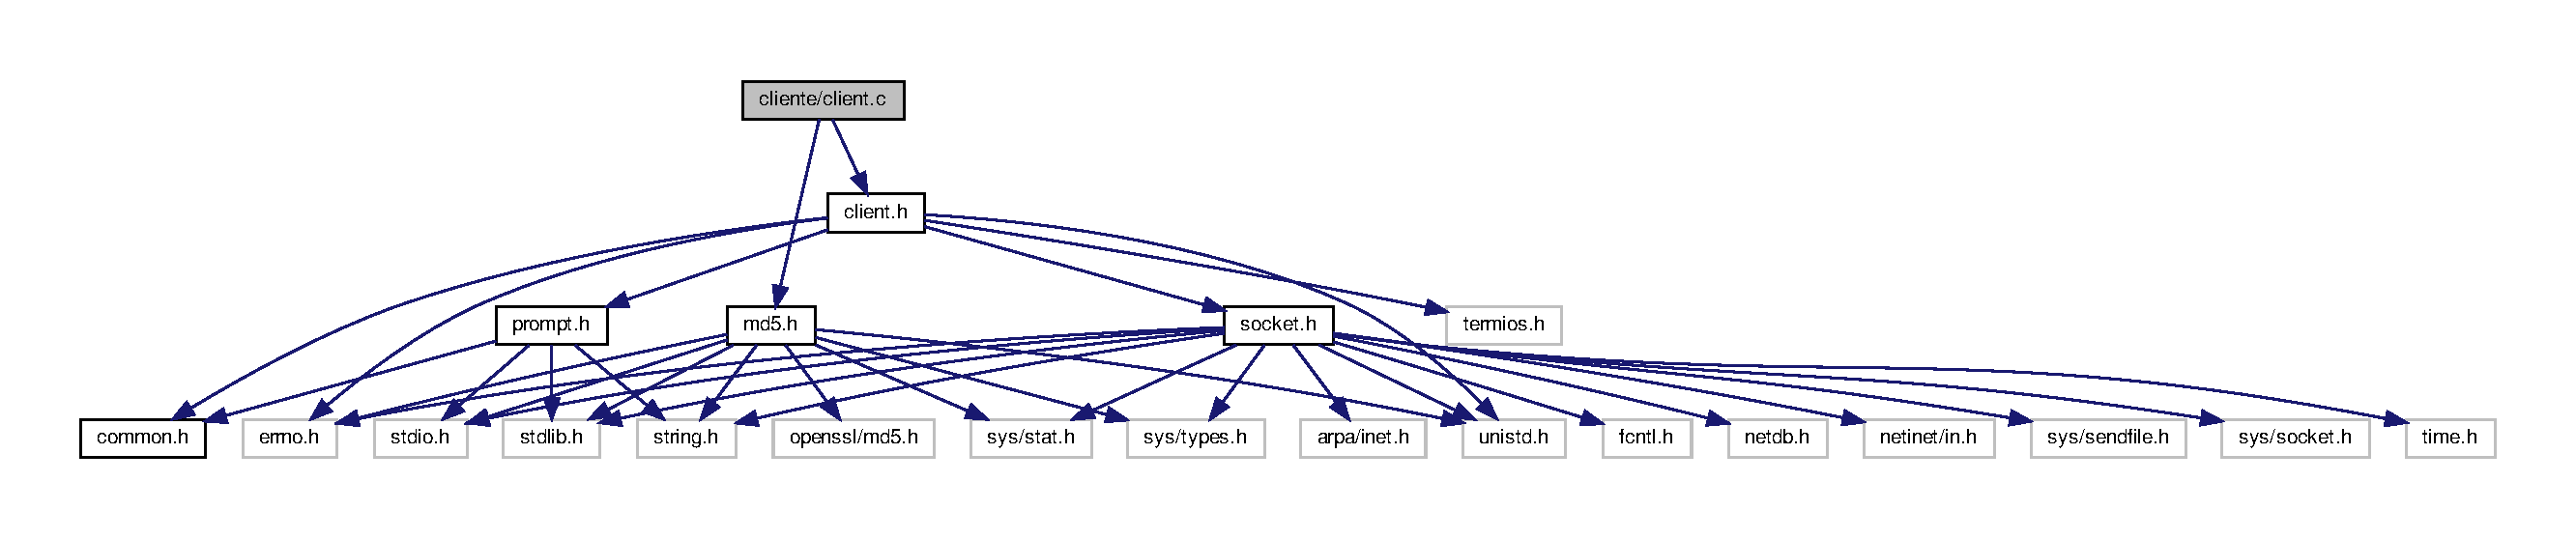
\includegraphics[width=350pt]{client_8c__incl}
\end{center}
\end{figure}
\subsection*{Functions}
\begin{DoxyCompactItemize}
\item 
char $\ast$ \textbf{ login} (char $\ast$userpass)
\begin{DoxyCompactList}\small\item\em Prompt for userpass ingress. \end{DoxyCompactList}\item 
int \textbf{ check\+\_\+status} (int status)
\begin{DoxyCompactList}\small\item\em Check if status if 0. \end{DoxyCompactList}\item 
void \textbf{ login\+\_\+handler} (int sockfd)
\begin{DoxyCompactList}\small\item\em The connection between the server and the client is handled from this function, which is also responsible for the message passage between these. \end{DoxyCompactList}\item 
void \textbf{ send\+\_\+cmd} (int sockfd, char $\ast$cmd)
\item 
int \textbf{ main} ()
\end{DoxyCompactItemize}


\subsection{Function Documentation}
\mbox{\label{client_8c_af00002a7d3df82f54b2041a687797915}} 
\index{client.\+c@{client.\+c}!check\+\_\+status@{check\+\_\+status}}
\index{check\+\_\+status@{check\+\_\+status}!client.\+c@{client.\+c}}
\subsubsection{check\+\_\+status()}
{\footnotesize\ttfamily int check\+\_\+status (\begin{DoxyParamCaption}\item[{int}]{status }\end{DoxyParamCaption})}



Check if status if 0. 


\begin{DoxyParams}{Parameters}
{\em status} & \\
\hline
\end{DoxyParams}
\begin{DoxyReturn}{Returns}
status 
\end{DoxyReturn}
\mbox{\label{client_8c_a0d2a952bfee88348e1792d66acf01e38}} 
\index{client.\+c@{client.\+c}!login@{login}}
\index{login@{login}!client.\+c@{client.\+c}}
\subsubsection{login()}
{\footnotesize\ttfamily char$\ast$ login (\begin{DoxyParamCaption}\item[{char $\ast$}]{userpass }\end{DoxyParamCaption})}



Prompt for userpass ingress. 


\begin{DoxyParams}{Parameters}
{\em userpass} & \\
\hline
\end{DoxyParams}
\begin{DoxyReturn}{Returns}
userpass 
\end{DoxyReturn}
\mbox{\label{client_8c_a471ae164131962c0fe21a47e23706139}} 
\index{client.\+c@{client.\+c}!login\+\_\+handler@{login\+\_\+handler}}
\index{login\+\_\+handler@{login\+\_\+handler}!client.\+c@{client.\+c}}
\subsubsection{login\+\_\+handler()}
{\footnotesize\ttfamily void login\+\_\+handler (\begin{DoxyParamCaption}\item[{int}]{sockfd }\end{DoxyParamCaption})}



The connection between the server and the client is handled from this function, which is also responsible for the message passage between these. 


\begin{DoxyParams}{Parameters}
{\em sockfd} & \\
\hline
\end{DoxyParams}
\mbox{\label{client_8c_ae66f6b31b5ad750f1fe042a706a4e3d4}} 
\index{client.\+c@{client.\+c}!main@{main}}
\index{main@{main}!client.\+c@{client.\+c}}
\subsubsection{main()}
{\footnotesize\ttfamily int main (\begin{DoxyParamCaption}\item[{void}]{ }\end{DoxyParamCaption})}

\mbox{\label{client_8c_a4117102389756aee8467678b28f484ed}} 
\index{client.\+c@{client.\+c}!send\+\_\+cmd@{send\+\_\+cmd}}
\index{send\+\_\+cmd@{send\+\_\+cmd}!client.\+c@{client.\+c}}
\subsubsection{send\+\_\+cmd()}
{\footnotesize\ttfamily void send\+\_\+cmd (\begin{DoxyParamCaption}\item[{int}]{sockfd,  }\item[{char $\ast$}]{cmd }\end{DoxyParamCaption})}


\section{cliente/prompt.c File Reference}
\label{prompt_8c}\index{cliente/prompt.\+c@{cliente/prompt.\+c}}
{\ttfamily \#include \char`\"{}prompt.\+h\char`\"{}}\newline
Include dependency graph for prompt.\+c\+:\nopagebreak
\begin{figure}[H]
\begin{center}
\leavevmode
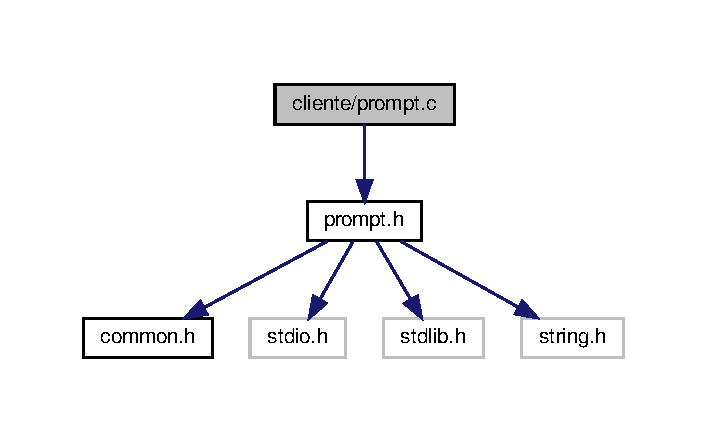
\includegraphics[width=340pt]{prompt_8c__incl}
\end{center}
\end{figure}
\subsection*{Functions}
\begin{DoxyCompactItemize}
\item 
char $\ast$ \textbf{ read\+\_\+line} (void)
\begin{DoxyCompactList}\small\item\em read line from stdin \end{DoxyCompactList}\item 
char $\ast$$\ast$ \textbf{ split\+\_\+line} (char $\ast$line)
\item 
int \textbf{ argc} (char $\ast$$\ast$n)
\begin{DoxyCompactList}\small\item\em Count the number of strings in a string array. \end{DoxyCompactList}\item 
int \textbf{ get\+\_\+cmd} (char $\ast$$\ast$args, int n\+\_\+args)
\begin{DoxyCompactList}\small\item\em Select type of command. \end{DoxyCompactList}\item 
char $\ast$ \textbf{ cmd\+\_\+prompt} (char $\ast$str\+\_\+to\+\_\+server)
\begin{DoxyCompactList}\small\item\em Prompt for the user. \end{DoxyCompactList}\item 
int \textbf{ is\+\_\+exit} (char $\ast$str)
\begin{DoxyCompactList}\small\item\em In case of the user has selected the exit command, then exit the prompt. \end{DoxyCompactList}\end{DoxyCompactItemize}


\subsection{Function Documentation}
\mbox{\label{prompt_8c_a29367ea7e75861b6b3db15e6d3a030ce}} 
\index{prompt.\+c@{prompt.\+c}!argc@{argc}}
\index{argc@{argc}!prompt.\+c@{prompt.\+c}}
\subsubsection{argc()}
{\footnotesize\ttfamily int argc (\begin{DoxyParamCaption}\item[{char $\ast$$\ast$}]{n }\end{DoxyParamCaption})}



Count the number of strings in a string array. 


\begin{DoxyParams}{Parameters}
{\em n} & array of strings \\
\hline
\end{DoxyParams}
\begin{DoxyReturn}{Returns}
number of strings 
\end{DoxyReturn}
\mbox{\label{prompt_8c_ac78cdc81595d63a0c876d3e3e8d2db70}} 
\index{prompt.\+c@{prompt.\+c}!cmd\+\_\+prompt@{cmd\+\_\+prompt}}
\index{cmd\+\_\+prompt@{cmd\+\_\+prompt}!prompt.\+c@{prompt.\+c}}
\subsubsection{cmd\+\_\+prompt()}
{\footnotesize\ttfamily char$\ast$ cmd\+\_\+prompt (\begin{DoxyParamCaption}\item[{char $\ast$}]{str\+\_\+to\+\_\+server }\end{DoxyParamCaption})}



Prompt for the user. 

All possibilities are contemplated to achieve robust behavior of the function. This may make it look a bit complex but it is properly documented for understanding the code. 
\begin{DoxyParams}{Parameters}
{\em str\+\_\+to\+\_\+server} & String to be sent to the server \\
\hline
\end{DoxyParams}
\begin{DoxyReturn}{Returns}
pointer to string  
\end{DoxyReturn}
Start of the prompt, it is kept in a do-\/while loop until the user enters a valid command.\mbox{\label{prompt_8c_a4eab3617254ab77fc2a44c5ff882f5f3}} 
\index{prompt.\+c@{prompt.\+c}!get\+\_\+cmd@{get\+\_\+cmd}}
\index{get\+\_\+cmd@{get\+\_\+cmd}!prompt.\+c@{prompt.\+c}}
\subsubsection{get\+\_\+cmd()}
{\footnotesize\ttfamily int get\+\_\+cmd (\begin{DoxyParamCaption}\item[{char $\ast$$\ast$}]{args,  }\item[{int}]{n\+\_\+args }\end{DoxyParamCaption})}



Select type of command. 

In case the first argument is any of the valid commands, the function will return an int greater than or equal to zero. If not it will return a negative int. 
\begin{DoxyParams}{Parameters}
{\em args} & Array of tokenized strings coming from user prompt \\
\hline
{\em n\+\_\+args} & Number of elements of array args \\
\hline
\end{DoxyParams}
\begin{DoxyReturn}{Returns}
int 
\end{DoxyReturn}
\mbox{\label{prompt_8c_a9882fc592454588fc3587f2ec03e09ab}} 
\index{prompt.\+c@{prompt.\+c}!is\+\_\+exit@{is\+\_\+exit}}
\index{is\+\_\+exit@{is\+\_\+exit}!prompt.\+c@{prompt.\+c}}
\subsubsection{is\+\_\+exit()}
{\footnotesize\ttfamily int is\+\_\+exit (\begin{DoxyParamCaption}\item[{char $\ast$}]{str }\end{DoxyParamCaption})}



In case of the user has selected the exit command, then exit the prompt. 


\begin{DoxyParams}{Parameters}
{\em str} & str\+\_\+to\+\_\+server \\
\hline
\end{DoxyParams}
\begin{DoxyReturn}{Returns}
int 
\end{DoxyReturn}
\mbox{\label{prompt_8c_ac14a4d3d27ec36419b82f72342be3a65}} 
\index{prompt.\+c@{prompt.\+c}!read\+\_\+line@{read\+\_\+line}}
\index{read\+\_\+line@{read\+\_\+line}!prompt.\+c@{prompt.\+c}}
\subsubsection{read\+\_\+line()}
{\footnotesize\ttfamily char$\ast$ read\+\_\+line (\begin{DoxyParamCaption}\item[{void}]{ }\end{DoxyParamCaption})}



read line from stdin 

\begin{DoxyReturn}{Returns}
char $\ast$ with the line 
\end{DoxyReturn}
\mbox{\label{prompt_8c_a0fa6791564b78ce51a5c31ddd923b892}} 
\index{prompt.\+c@{prompt.\+c}!split\+\_\+line@{split\+\_\+line}}
\index{split\+\_\+line@{split\+\_\+line}!prompt.\+c@{prompt.\+c}}
\subsubsection{split\+\_\+line()}
{\footnotesize\ttfamily char$\ast$$\ast$ split\+\_\+line (\begin{DoxyParamCaption}\item[{char $\ast$}]{line }\end{DoxyParamCaption})}


\begin{DoxyParams}{Parameters}
{\em line} & \\
\hline
\end{DoxyParams}
\begin{DoxyReturn}{Returns}
char$\ast$$\ast$ 
\end{DoxyReturn}

\section{cliente/socket\+\_\+client.c File Reference}
\label{socket__client_8c}\index{cliente/socket\+\_\+client.\+c@{cliente/socket\+\_\+client.\+c}}
{\ttfamily \#include \char`\"{}socket.\+h\char`\"{}}\newline
{\ttfamily \#include \char`\"{}common.\+h\char`\"{}}\newline
{\ttfamily \#include $<$unistd.\+h$>$}\newline
Include dependency graph for socket\+\_\+client.\+c\+:
\nopagebreak
\begin{figure}[H]
\begin{center}
\leavevmode
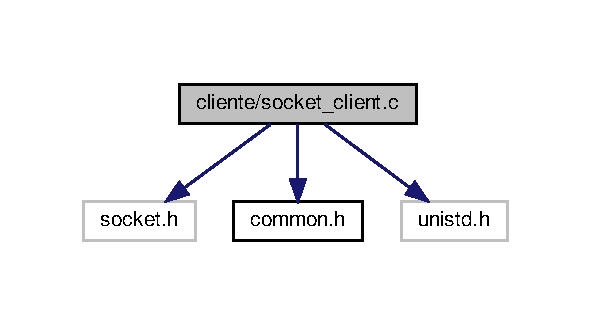
\includegraphics[width=284pt]{socket__client_8c__incl}
\end{center}
\end{figure}
\subsection*{Functions}
\begin{DoxyCompactItemize}
\item 
int \textbf{ cli\+\_\+socket} (int port)
\begin{DoxyCompactList}\small\item\em Creation, assign IP and port of client socket. Connect to server is included. \end{DoxyCompactList}\item 
long int \textbf{ recv\+\_\+file} (int newsockfd, int fd)
\begin{DoxyCompactList}\small\item\em The file is received from the fileserver through a socket. \end{DoxyCompactList}\item 
long int \textbf{ transfer\+\_\+file} (int newsockfd, char $\ast$usb)
\begin{DoxyCompactList}\small\item\em File is created and proceeds to receive while the transfer time is calculated. \end{DoxyCompactList}\end{DoxyCompactItemize}


\subsection{Function Documentation}
\mbox{\label{socket__client_8c_ad00c6fbc3ed7bc44f4e78ad434174830}} 
\index{socket\+\_\+client.\+c@{socket\+\_\+client.\+c}!cli\+\_\+socket@{cli\+\_\+socket}}
\index{cli\+\_\+socket@{cli\+\_\+socket}!socket\+\_\+client.\+c@{socket\+\_\+client.\+c}}
\subsubsection{cli\+\_\+socket()}
{\footnotesize\ttfamily int cli\+\_\+socket (\begin{DoxyParamCaption}\item[{int}]{port }\end{DoxyParamCaption})}



Creation, assign IP and port of client socket. Connect to server is included. 

\begin{DoxyReturn}{Returns}
sockfd 
\end{DoxyReturn}
\mbox{\label{socket__client_8c_a621d70c2ed3ab16e2bc0c9ec45b390ce}} 
\index{socket\+\_\+client.\+c@{socket\+\_\+client.\+c}!recv\+\_\+file@{recv\+\_\+file}}
\index{recv\+\_\+file@{recv\+\_\+file}!socket\+\_\+client.\+c@{socket\+\_\+client.\+c}}
\subsubsection{recv\+\_\+file()}
{\footnotesize\ttfamily long int recv\+\_\+file (\begin{DoxyParamCaption}\item[{int}]{newsockfd,  }\item[{int}]{fd }\end{DoxyParamCaption})}



The file is received from the fileserver through a socket. 


\begin{DoxyParams}{Parameters}
{\em newsockfd} & \\
\hline
{\em fd} & \\
\hline
\end{DoxyParams}
\mbox{\label{socket__client_8c_a0b59c96534746c30c167f090497a8dd0}} 
\index{socket\+\_\+client.\+c@{socket\+\_\+client.\+c}!transfer\+\_\+file@{transfer\+\_\+file}}
\index{transfer\+\_\+file@{transfer\+\_\+file}!socket\+\_\+client.\+c@{socket\+\_\+client.\+c}}
\subsubsection{transfer\+\_\+file()}
{\footnotesize\ttfamily long int transfer\+\_\+file (\begin{DoxyParamCaption}\item[{int}]{newsockfd,  }\item[{char $\ast$}]{usb }\end{DoxyParamCaption})}



File is created and proceeds to receive while the transfer time is calculated. 


\begin{DoxyParams}{Parameters}
{\em newsockfd} & \\
\hline
\end{DoxyParams}

\section{include/auth.h File Reference}
\label{auth_8h}\index{include/auth.\+h@{include/auth.\+h}}
{\ttfamily \#include \char`\"{}common.\+h\char`\"{}}\newline
{\ttfamily \#include $<$stdio.\+h$>$}\newline
{\ttfamily \#include $<$string.\+h$>$}\newline
{\ttfamily \#include $<$stdlib.\+h$>$}\newline
{\ttfamily \#include $<$errno.\+h$>$}\newline
{\ttfamily \#include $<$time.\+h$>$}\newline
Include dependency graph for auth.\+h\+:\nopagebreak
\begin{figure}[H]
\begin{center}
\leavevmode
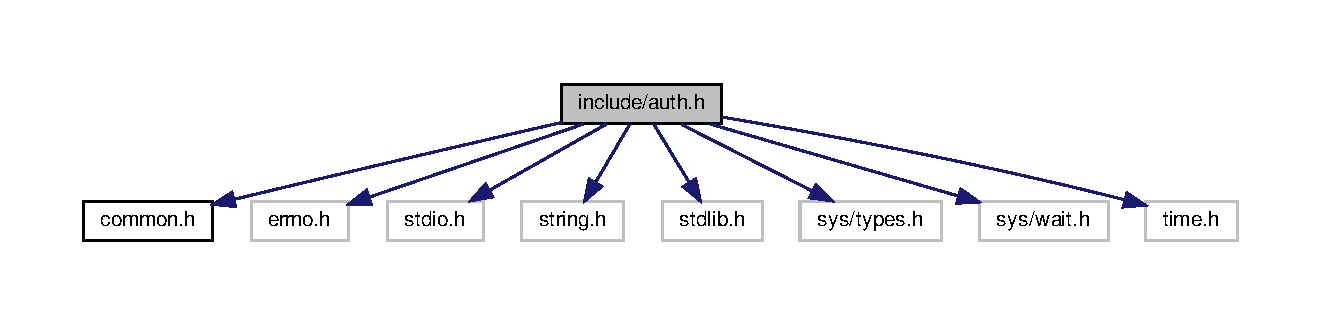
\includegraphics[width=350pt]{auth_8h__incl}
\end{center}
\end{figure}
This graph shows which files directly or indirectly include this file\+:\nopagebreak
\begin{figure}[H]
\begin{center}
\leavevmode
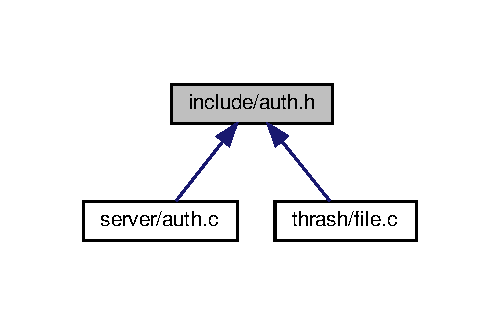
\includegraphics[width=240pt]{auth_8h__dep__incl}
\end{center}
\end{figure}
\subsection*{Data Structures}
\begin{DoxyCompactItemize}
\item 
struct \textbf{ user}
\end{DoxyCompactItemize}
\subsection*{Macros}
\begin{DoxyCompactItemize}
\item 
\#define \textbf{ P\+O\+R\+T\+\_\+\+F\+LS}~10001
\item 
\#define \textbf{ U\+S\+E\+RS}~3
\end{DoxyCompactItemize}
\subsection*{Functions}
\begin{DoxyCompactItemize}
\item 
void \textbf{ change\+\_\+pass} (char $\ast$, char $\ast$)
\begin{DoxyCompactList}\small\item\em Change user pass in DB. \end{DoxyCompactList}\item 
int \textbf{ check\+\_\+block} (char $\ast$)
\begin{DoxyCompactList}\small\item\em Check the number of user blocks. \end{DoxyCompactList}\item 
int \textbf{ cmd\+\_\+handler} (int, char $\ast$)
\begin{DoxyCompactList}\small\item\em Login handler between [A\+UT] and [S\+RV]. \end{DoxyCompactList}\item 
void \textbf{ increase\+\_\+block} (char $\ast$)
\begin{DoxyCompactList}\small\item\em Increase number of blocks according to user. \end{DoxyCompactList}\item 
char $\ast$ \textbf{ get\+\_\+pass} (char $\ast$)
\begin{DoxyCompactList}\small\item\em Returns the pass substr of str. \end{DoxyCompactList}\item 
int \textbf{ get\+\_\+status} (char $\ast$, char $\ast$)
\begin{DoxyCompactList}\small\item\em Get the status of check userpass. \end{DoxyCompactList}\item 
void \textbf{ last\+\_\+connect} (char $\ast$)
\begin{DoxyCompactList}\small\item\em Registers the date of the login of a user saving the value in the database. \end{DoxyCompactList}\item 
char $\ast$ \textbf{ list\+\_\+users} (char $\ast$)
\begin{DoxyCompactList}\small\item\em List users in DB. \end{DoxyCompactList}\item 
void \textbf{ load\+\_\+db} (void)
\begin{DoxyCompactList}\small\item\em Load users to DB from C\+SV file. \end{DoxyCompactList}\item 
char $\ast$ \textbf{ login\+\_\+handler} (int, char $\ast$)
\begin{DoxyCompactList}\small\item\em Login handler between auth and srv. \end{DoxyCompactList}\item 
void \textbf{ save\+\_\+db} (void)
\begin{DoxyCompactList}\small\item\em Save DB changes in C\+SV file. \end{DoxyCompactList}\end{DoxyCompactItemize}
\subsection*{Variables}
\begin{DoxyCompactItemize}
\item 
struct \textbf{ user} \textbf{ users} [\textbf{ U\+S\+E\+RS}]
\end{DoxyCompactItemize}


\subsection{Macro Definition Documentation}
\mbox{\label{auth_8h_a618d6577d85428a5a48d41a23c107555}} 
\index{auth.\+h@{auth.\+h}!P\+O\+R\+T\+\_\+\+F\+LS@{P\+O\+R\+T\+\_\+\+F\+LS}}
\index{P\+O\+R\+T\+\_\+\+F\+LS@{P\+O\+R\+T\+\_\+\+F\+LS}!auth.\+h@{auth.\+h}}
\subsubsection{P\+O\+R\+T\+\_\+\+F\+LS}
{\footnotesize\ttfamily \#define P\+O\+R\+T\+\_\+\+F\+LS~10001}

\mbox{\label{auth_8h_a322789c10f93ef5e09a1d5f17aabf0e3}} 
\index{auth.\+h@{auth.\+h}!U\+S\+E\+RS@{U\+S\+E\+RS}}
\index{U\+S\+E\+RS@{U\+S\+E\+RS}!auth.\+h@{auth.\+h}}
\subsubsection{U\+S\+E\+RS}
{\footnotesize\ttfamily \#define U\+S\+E\+RS~3}



\subsection{Function Documentation}
\mbox{\label{auth_8h_a97aeb8e1fb29fa958c8ea862bda5ba69}} 
\index{auth.\+h@{auth.\+h}!change\+\_\+pass@{change\+\_\+pass}}
\index{change\+\_\+pass@{change\+\_\+pass}!auth.\+h@{auth.\+h}}
\subsubsection{change\+\_\+pass()}
{\footnotesize\ttfamily void change\+\_\+pass (\begin{DoxyParamCaption}\item[{char $\ast$}]{user,  }\item[{char $\ast$}]{pass }\end{DoxyParamCaption})}



Change user pass in DB. 


\begin{DoxyParams}{Parameters}
{\em user} & \\
\hline
{\em pass} & \\
\hline
\end{DoxyParams}
\mbox{\label{auth_8h_a3bf3271f2878741a36a522714fc1180b}} 
\index{auth.\+h@{auth.\+h}!check\+\_\+block@{check\+\_\+block}}
\index{check\+\_\+block@{check\+\_\+block}!auth.\+h@{auth.\+h}}
\subsubsection{check\+\_\+block()}
{\footnotesize\ttfamily int check\+\_\+block (\begin{DoxyParamCaption}\item[{char $\ast$}]{user }\end{DoxyParamCaption})}



Check the number of user blocks. 


\begin{DoxyParams}{Parameters}
{\em user} & \\
\hline
\end{DoxyParams}
\begin{DoxyReturn}{Returns}
int 1 if user have 3 or more blocks else 0 
\end{DoxyReturn}
\mbox{\label{auth_8h_ac577f045e4bf8abe2128eb727bf5edb7}} 
\index{auth.\+h@{auth.\+h}!cmd\+\_\+handler@{cmd\+\_\+handler}}
\index{cmd\+\_\+handler@{cmd\+\_\+handler}!auth.\+h@{auth.\+h}}
\subsubsection{cmd\+\_\+handler()}
{\footnotesize\ttfamily int cmd\+\_\+handler (\begin{DoxyParamCaption}\item[{int}]{msqid,  }\item[{char $\ast$}]{user }\end{DoxyParamCaption})}



Login handler between [A\+UT] and [S\+RV]. 


\begin{DoxyParams}{Parameters}
{\em msqid} & \\
\hline
\end{DoxyParams}
\mbox{\label{auth_8h_ab699bd210dfe5219d858aeb212650f47}} 
\index{auth.\+h@{auth.\+h}!get\+\_\+pass@{get\+\_\+pass}}
\index{get\+\_\+pass@{get\+\_\+pass}!auth.\+h@{auth.\+h}}
\subsubsection{get\+\_\+pass()}
{\footnotesize\ttfamily char$\ast$ get\+\_\+pass (\begin{DoxyParamCaption}\item[{char $\ast$}]{str }\end{DoxyParamCaption})}



Returns the pass substr of str. 


\begin{DoxyParams}{Parameters}
{\em str} & \\
\hline
\end{DoxyParams}
\begin{DoxyReturn}{Returns}
char$\ast$ 
\end{DoxyReturn}
\mbox{\label{auth_8h_ac2d257768c5b44d17c6fe989707468a5}} 
\index{auth.\+h@{auth.\+h}!get\+\_\+status@{get\+\_\+status}}
\index{get\+\_\+status@{get\+\_\+status}!auth.\+h@{auth.\+h}}
\subsubsection{get\+\_\+status()}
{\footnotesize\ttfamily int get\+\_\+status (\begin{DoxyParamCaption}\item[{char $\ast$}]{userpass,  }\item[{char $\ast$}]{user }\end{DoxyParamCaption})}



Get the status of check userpass. 


\begin{DoxyParams}{Parameters}
{\em userpass} & \\
\hline
\end{DoxyParams}
\begin{DoxyReturn}{Returns}
int 1\+: user and pass correct 0\+: pass wrong -\/1\+: user wrong -\/2\+: user blocked 
\end{DoxyReturn}
\mbox{\label{auth_8h_a7262d58710ad875161637d4d2ae75009}} 
\index{auth.\+h@{auth.\+h}!increase\+\_\+block@{increase\+\_\+block}}
\index{increase\+\_\+block@{increase\+\_\+block}!auth.\+h@{auth.\+h}}
\subsubsection{increase\+\_\+block()}
{\footnotesize\ttfamily void increase\+\_\+block (\begin{DoxyParamCaption}\item[{char $\ast$}]{user }\end{DoxyParamCaption})}



Increase number of blocks according to user. 


\begin{DoxyParams}{Parameters}
{\em user} & \\
\hline
\end{DoxyParams}
\mbox{\label{auth_8h_a45125798b5e6b7446e4f699ff5d5ce7e}} 
\index{auth.\+h@{auth.\+h}!last\+\_\+connect@{last\+\_\+connect}}
\index{last\+\_\+connect@{last\+\_\+connect}!auth.\+h@{auth.\+h}}
\subsubsection{last\+\_\+connect()}
{\footnotesize\ttfamily void last\+\_\+connect (\begin{DoxyParamCaption}\item[{char $\ast$}]{user }\end{DoxyParamCaption})}



Registers the date of the login of a user saving the value in the database. 


\begin{DoxyParams}{Parameters}
{\em user} & \\
\hline
\end{DoxyParams}
\mbox{\label{auth_8h_aac12c870325e2f9d95be2cffb49abe78}} 
\index{auth.\+h@{auth.\+h}!list\+\_\+users@{list\+\_\+users}}
\index{list\+\_\+users@{list\+\_\+users}!auth.\+h@{auth.\+h}}
\subsubsection{list\+\_\+users()}
{\footnotesize\ttfamily char $\ast$ list\+\_\+users (\begin{DoxyParamCaption}\item[{char $\ast$}]{str\+Users }\end{DoxyParamCaption})}



List users in DB. 


\begin{DoxyParams}{Parameters}
{\em str\+Users} & \\
\hline
\end{DoxyParams}
\begin{DoxyReturn}{Returns}
char$\ast$ with users information 
\end{DoxyReturn}
\mbox{\label{auth_8h_aca138a298c612a14d6fb2c16672f8c87}} 
\index{auth.\+h@{auth.\+h}!load\+\_\+db@{load\+\_\+db}}
\index{load\+\_\+db@{load\+\_\+db}!auth.\+h@{auth.\+h}}
\subsubsection{load\+\_\+db()}
{\footnotesize\ttfamily void load\+\_\+db (\begin{DoxyParamCaption}\item[{void}]{ }\end{DoxyParamCaption})}



Load users to DB from C\+SV file. 

\mbox{\label{auth_8h_a83d64e63f624455cc546824658a42969}} 
\index{auth.\+h@{auth.\+h}!login\+\_\+handler@{login\+\_\+handler}}
\index{login\+\_\+handler@{login\+\_\+handler}!auth.\+h@{auth.\+h}}
\subsubsection{login\+\_\+handler()}
{\footnotesize\ttfamily char $\ast$ login\+\_\+handler (\begin{DoxyParamCaption}\item[{int}]{msqid,  }\item[{char $\ast$}]{user }\end{DoxyParamCaption})}



Login handler between auth and srv. 


\begin{DoxyParams}{Parameters}
{\em msqid} & \\
\hline
\end{DoxyParams}
\mbox{\label{auth_8h_a7145eb48ec5e46fbb39b0b174a026cd1}} 
\index{auth.\+h@{auth.\+h}!save\+\_\+db@{save\+\_\+db}}
\index{save\+\_\+db@{save\+\_\+db}!auth.\+h@{auth.\+h}}
\subsubsection{save\+\_\+db()}
{\footnotesize\ttfamily void save\+\_\+db (\begin{DoxyParamCaption}\item[{void}]{ }\end{DoxyParamCaption})}



Save DB changes in C\+SV file. 



\subsection{Variable Documentation}
\mbox{\label{auth_8h_ad1b6438b2448da2b01d9887f58f5fb66}} 
\index{auth.\+h@{auth.\+h}!users@{users}}
\index{users@{users}!auth.\+h@{auth.\+h}}
\subsubsection{users}
{\footnotesize\ttfamily struct \textbf{ user} users[\textbf{ U\+S\+E\+RS}]}


\section{include/client.h File Reference}
\label{client_8h}\index{include/client.\+h@{include/client.\+h}}
{\ttfamily \#include \char`\"{}socket.\+h\char`\"{}}\newline
{\ttfamily \#include \char`\"{}prompt.\+h\char`\"{}}\newline
{\ttfamily \#include \char`\"{}common.\+h\char`\"{}}\newline
{\ttfamily \#include $<$errno.\+h$>$}\newline
{\ttfamily \#include $<$termios.\+h$>$}\newline
{\ttfamily \#include $<$unistd.\+h$>$}\newline
Include dependency graph for client.\+h\+:\nopagebreak
\begin{figure}[H]
\begin{center}
\leavevmode
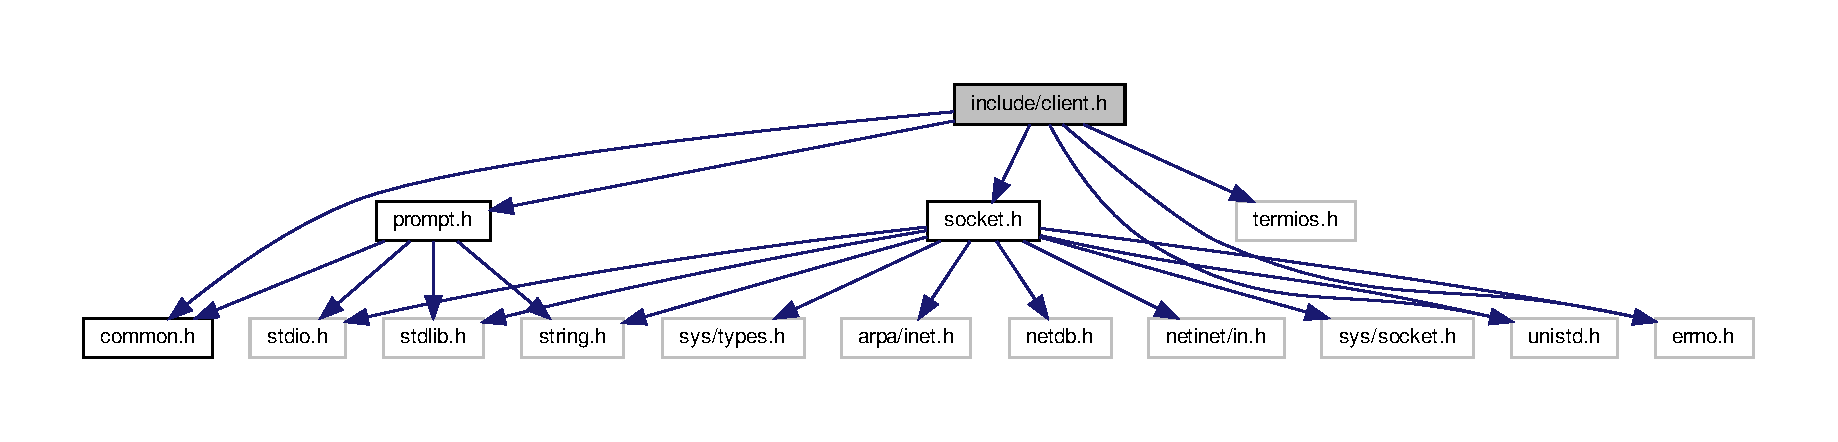
\includegraphics[width=350pt]{client_8h__incl}
\end{center}
\end{figure}
This graph shows which files directly or indirectly include this file\+:\nopagebreak
\begin{figure}[H]
\begin{center}
\leavevmode
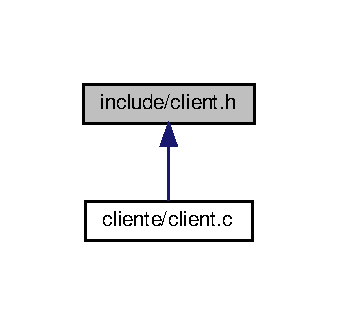
\includegraphics[width=162pt]{client_8h__dep__incl}
\end{center}
\end{figure}
\subsection*{Functions}
\begin{DoxyCompactItemize}
\item 
void \textbf{ burn\+\_\+usb} (char $\ast$, char $\ast$)
\begin{DoxyCompactList}\small\item\em Send the image to the U\+SB. \end{DoxyCompactList}\item 
int \textbf{ check\+\_\+status} (int)
\begin{DoxyCompactList}\small\item\em Check status. \end{DoxyCompactList}\item 
void \textbf{ file\+\_\+down} (void)
\begin{DoxyCompactList}\small\item\em If the image exists in the fileserver, it receives, saves, burns, erases and calculates the md5 and M\+BR of the U\+SB. \end{DoxyCompactList}\item 
char $\ast$ \textbf{ login} (char $\ast$)
\begin{DoxyCompactList}\small\item\em Prompt for userpass ingress. \end{DoxyCompactList}\item 
void \textbf{ login\+\_\+handler} (int)
\begin{DoxyCompactList}\small\item\em The connection between the server and the client is handled from this function, which is also responsible for the message passage between these. \end{DoxyCompactList}\item 
void \textbf{ send\+\_\+cmd} (int, char $\ast$)
\begin{DoxyCompactList}\small\item\em Send message to the server through a socket. \end{DoxyCompactList}\end{DoxyCompactItemize}


\subsection{Function Documentation}
\mbox{\label{client_8h_a8f5170bbb9c0c247151775f99a577ff5}} 
\index{client.\+h@{client.\+h}!burn\+\_\+usb@{burn\+\_\+usb}}
\index{burn\+\_\+usb@{burn\+\_\+usb}!client.\+h@{client.\+h}}
\subsubsection{burn\+\_\+usb()}
{\footnotesize\ttfamily void burn\+\_\+usb (\begin{DoxyParamCaption}\item[{char $\ast$}]{img,  }\item[{char $\ast$}]{usb }\end{DoxyParamCaption})}



Send the image to the U\+SB. 


\begin{DoxyParams}{Parameters}
{\em img} & \\
\hline
{\em usb} & \\
\hline
\end{DoxyParams}
\mbox{\label{client_8h_af8b753753a0d32bcef5a40e1a49b7a18}} 
\index{client.\+h@{client.\+h}!check\+\_\+status@{check\+\_\+status}}
\index{check\+\_\+status@{check\+\_\+status}!client.\+h@{client.\+h}}
\subsubsection{check\+\_\+status()}
{\footnotesize\ttfamily int check\+\_\+status (\begin{DoxyParamCaption}\item[{int}]{status }\end{DoxyParamCaption})}



Check status. 


\begin{DoxyParams}{Parameters}
{\em status} & \\
\hline
\end{DoxyParams}
\begin{DoxyReturn}{Returns}
status 
\end{DoxyReturn}
\mbox{\label{client_8h_aacd5c156cb2388028cddb5242f1fe5c2}} 
\index{client.\+h@{client.\+h}!file\+\_\+down@{file\+\_\+down}}
\index{file\+\_\+down@{file\+\_\+down}!client.\+h@{client.\+h}}
\subsubsection{file\+\_\+down()}
{\footnotesize\ttfamily void file\+\_\+down (\begin{DoxyParamCaption}\item[{void}]{ }\end{DoxyParamCaption})}



If the image exists in the fileserver, it receives, saves, burns, erases and calculates the md5 and M\+BR of the U\+SB. 

\mbox{\label{client_8h_a184b4ae1814dc2cdcea053bafd7f097f}} 
\index{client.\+h@{client.\+h}!login@{login}}
\index{login@{login}!client.\+h@{client.\+h}}
\subsubsection{login()}
{\footnotesize\ttfamily char$\ast$ login (\begin{DoxyParamCaption}\item[{char $\ast$}]{userpass }\end{DoxyParamCaption})}



Prompt for userpass ingress. 


\begin{DoxyParams}{Parameters}
{\em userpass} & \\
\hline
\end{DoxyParams}
\begin{DoxyReturn}{Returns}
userpass 
\end{DoxyReturn}
\mbox{\label{client_8h_a98d7f4c6baab897a754ea7a006c5cb11}} 
\index{client.\+h@{client.\+h}!login\+\_\+handler@{login\+\_\+handler}}
\index{login\+\_\+handler@{login\+\_\+handler}!client.\+h@{client.\+h}}
\subsubsection{login\+\_\+handler()}
{\footnotesize\ttfamily void login\+\_\+handler (\begin{DoxyParamCaption}\item[{int}]{sockfd }\end{DoxyParamCaption})}



The connection between the server and the client is handled from this function, which is also responsible for the message passage between these. 


\begin{DoxyParams}{Parameters}
{\em sockfd} & \\
\hline
\end{DoxyParams}
\mbox{\label{client_8h_a3f2e03899acbcffa63c626522bfb6c40}} 
\index{client.\+h@{client.\+h}!send\+\_\+cmd@{send\+\_\+cmd}}
\index{send\+\_\+cmd@{send\+\_\+cmd}!client.\+h@{client.\+h}}
\subsubsection{send\+\_\+cmd()}
{\footnotesize\ttfamily void send\+\_\+cmd (\begin{DoxyParamCaption}\item[{int}]{sockfd,  }\item[{char $\ast$}]{cmd }\end{DoxyParamCaption})}



Send message to the server through a socket. 


\begin{DoxyParams}{Parameters}
{\em sockfd} & \\
\hline
{\em cmd} & \\
\hline
\end{DoxyParams}

\section{include/common.h File Reference}
\label{common_8h}\index{include/common.\+h@{include/common.\+h}}
This graph shows which files directly or indirectly include this file\+:
\nopagebreak
\begin{figure}[H]
\begin{center}
\leavevmode
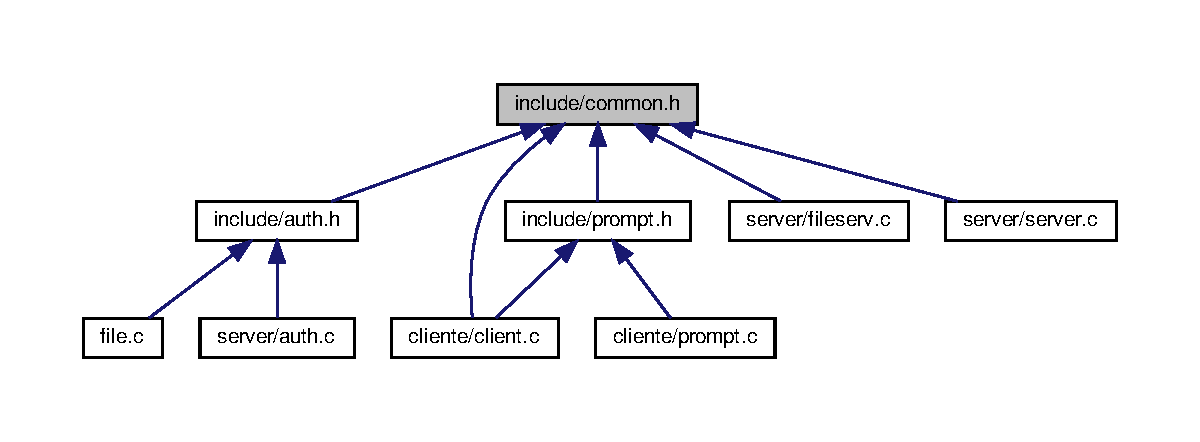
\includegraphics[width=350pt]{common_8h__dep__incl}
\end{center}
\end{figure}
\subsection*{Macros}
\begin{DoxyCompactItemize}
\item 
\#define \textbf{ auth\+\_\+type}~1
\item 
\#define \textbf{ files\+\_\+type}~2
\item 
\#define \textbf{ B\+U\+F\+F\+S\+I\+ZE}~1024
\item 
\#define \textbf{ D\+E\+B\+UG}~1
\item 
\#define \textbf{ L\+O\+G\+IN}~1
\item 
\#define \textbf{ P\+O\+R\+T\+\_\+\+S\+RV}~10004
\end{DoxyCompactItemize}


\subsection{Macro Definition Documentation}
\mbox{\label{common_8h_aeccf496f78c1193cbacd50d37bf8fa2d}} 
\index{common.\+h@{common.\+h}!auth\+\_\+type@{auth\+\_\+type}}
\index{auth\+\_\+type@{auth\+\_\+type}!common.\+h@{common.\+h}}
\subsubsection{auth\+\_\+type}
{\footnotesize\ttfamily \#define auth\+\_\+type~1}

\mbox{\label{common_8h_a39912bfe2a55f30e269196f9141d845d}} 
\index{common.\+h@{common.\+h}!B\+U\+F\+F\+S\+I\+ZE@{B\+U\+F\+F\+S\+I\+ZE}}
\index{B\+U\+F\+F\+S\+I\+ZE@{B\+U\+F\+F\+S\+I\+ZE}!common.\+h@{common.\+h}}
\subsubsection{B\+U\+F\+F\+S\+I\+ZE}
{\footnotesize\ttfamily \#define B\+U\+F\+F\+S\+I\+ZE~1024}

\mbox{\label{common_8h_ad72dbcf6d0153db1b8d8a58001feed83}} 
\index{common.\+h@{common.\+h}!D\+E\+B\+UG@{D\+E\+B\+UG}}
\index{D\+E\+B\+UG@{D\+E\+B\+UG}!common.\+h@{common.\+h}}
\subsubsection{D\+E\+B\+UG}
{\footnotesize\ttfamily \#define D\+E\+B\+UG~1}

\mbox{\label{common_8h_a06ecdafe3df3478eab750a18f6f8371d}} 
\index{common.\+h@{common.\+h}!files\+\_\+type@{files\+\_\+type}}
\index{files\+\_\+type@{files\+\_\+type}!common.\+h@{common.\+h}}
\subsubsection{files\+\_\+type}
{\footnotesize\ttfamily \#define files\+\_\+type~2}

\mbox{\label{common_8h_a2cc44bf853cfd679b56807b198735596}} 
\index{common.\+h@{common.\+h}!L\+O\+G\+IN@{L\+O\+G\+IN}}
\index{L\+O\+G\+IN@{L\+O\+G\+IN}!common.\+h@{common.\+h}}
\subsubsection{L\+O\+G\+IN}
{\footnotesize\ttfamily \#define L\+O\+G\+IN~1}

\mbox{\label{common_8h_a63cc51955a32e949e602d322d28762ec}} 
\index{common.\+h@{common.\+h}!P\+O\+R\+T\+\_\+\+S\+RV@{P\+O\+R\+T\+\_\+\+S\+RV}}
\index{P\+O\+R\+T\+\_\+\+S\+RV@{P\+O\+R\+T\+\_\+\+S\+RV}!common.\+h@{common.\+h}}
\subsubsection{P\+O\+R\+T\+\_\+\+S\+RV}
{\footnotesize\ttfamily \#define P\+O\+R\+T\+\_\+\+S\+RV~10004}


\section{include/fileserv.h File Reference}
\label{fileserv_8h}\index{include/fileserv.\+h@{include/fileserv.\+h}}
{\ttfamily \#include \char`\"{}md5.\+h\char`\"{}}\newline
{\ttfamily \#include \char`\"{}mq.\+h\char`\"{}}\newline
{\ttfamily \#include \char`\"{}common.\+h\char`\"{}}\newline
{\ttfamily \#include \char`\"{}socket.\+h\char`\"{}}\newline
{\ttfamily \#include $<$dirent.\+h$>$}\newline
{\ttfamily \#include $<$stdio.\+h$>$}\newline
{\ttfamily \#include $<$stdlib.\+h$>$}\newline
{\ttfamily \#include $<$stdint.\+h$>$}\newline
{\ttfamily \#include $<$sys/stat.\+h$>$}\newline
{\ttfamily \#include $<$string.\+h$>$}\newline
{\ttfamily \#include $<$openssl/md5.\+h$>$}\newline
{\ttfamily \#include $<$errno.\+h$>$}\newline
Include dependency graph for fileserv.\+h\+:
\nopagebreak
\begin{figure}[H]
\begin{center}
\leavevmode
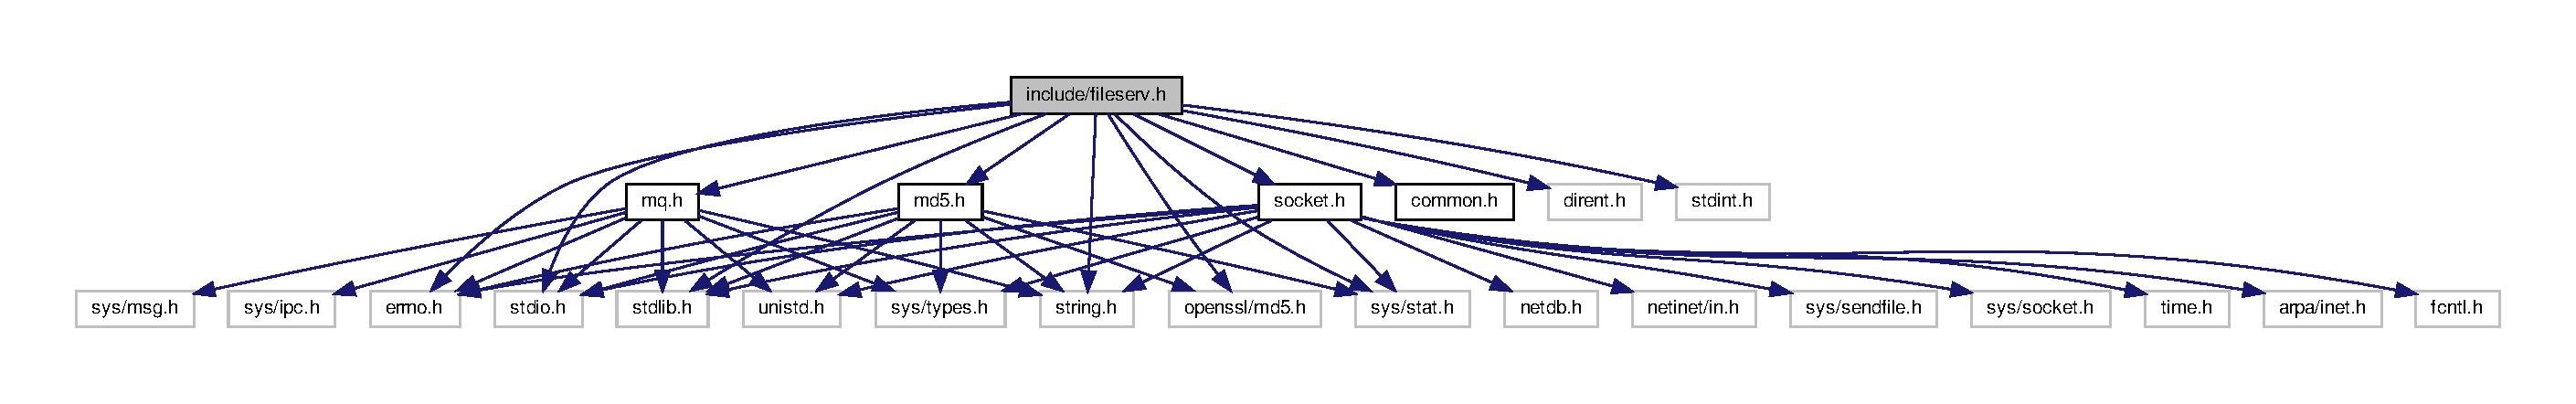
\includegraphics[width=350pt]{fileserv_8h__incl}
\end{center}
\end{figure}
This graph shows which files directly or indirectly include this file\+:
\nopagebreak
\begin{figure}[H]
\begin{center}
\leavevmode
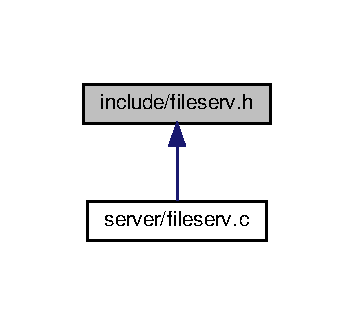
\includegraphics[width=170pt]{fileserv_8h__dep__incl}
\end{center}
\end{figure}
\subsection*{Functions}
\begin{DoxyCompactItemize}
\item 
int \textbf{ cmd\+\_\+handler} (int)
\begin{DoxyCompactList}\small\item\em Command handler. \end{DoxyCompactList}\item 
char $\ast$ \textbf{ files\+\_\+info} (char $\ast$)
\begin{DoxyCompactList}\small\item\em Collection of the required information for each file in a specific folder. \end{DoxyCompactList}\item 
char $\ast$ \textbf{ readable\+\_\+fs} (long int, char $\ast$)
\begin{DoxyCompactList}\small\item\em Parser that returns in human-\/readable format the size of a file. \end{DoxyCompactList}\end{DoxyCompactItemize}


\subsection{Function Documentation}
\mbox{\label{fileserv_8h_a17e3a23bd1ae378882eab0ef0f856de1}} 
\index{fileserv.\+h@{fileserv.\+h}!cmd\+\_\+handler@{cmd\+\_\+handler}}
\index{cmd\+\_\+handler@{cmd\+\_\+handler}!fileserv.\+h@{fileserv.\+h}}
\subsubsection{cmd\+\_\+handler()}
{\footnotesize\ttfamily int cmd\+\_\+handler (\begin{DoxyParamCaption}\item[{int}]{msqid }\end{DoxyParamCaption})}



Command handler. 


\begin{DoxyParams}{Parameters}
{\em msqid} & \\
\hline
\end{DoxyParams}
\begin{DoxyReturn}{Returns}
int exit
\end{DoxyReturn}
Command handler.


\begin{DoxyParams}{Parameters}
{\em msqid} & \\
\hline
\end{DoxyParams}
\mbox{\label{fileserv_8h_a49cfaf7b6d546c559fb0901bd5ba3e65}} 
\index{fileserv.\+h@{fileserv.\+h}!files\+\_\+info@{files\+\_\+info}}
\index{files\+\_\+info@{files\+\_\+info}!fileserv.\+h@{fileserv.\+h}}
\subsubsection{files\+\_\+info()}
{\footnotesize\ttfamily char$\ast$ files\+\_\+info (\begin{DoxyParamCaption}\item[{char $\ast$}]{files\+Info }\end{DoxyParamCaption})}



Collection of the required information for each file in a specific folder. 


\begin{DoxyParams}{Parameters}
{\em files\+Info} & \\
\hline
\end{DoxyParams}
\begin{DoxyReturn}{Returns}
Formatted string ready to be printed or sent 
\end{DoxyReturn}
\mbox{\label{fileserv_8h_aaa60420f4ed2522f7e58eedb72afea48}} 
\index{fileserv.\+h@{fileserv.\+h}!readable\+\_\+fs@{readable\+\_\+fs}}
\index{readable\+\_\+fs@{readable\+\_\+fs}!fileserv.\+h@{fileserv.\+h}}
\subsubsection{readable\+\_\+fs()}
{\footnotesize\ttfamily char$\ast$ readable\+\_\+fs (\begin{DoxyParamCaption}\item[{long int}]{size,  }\item[{char $\ast$}]{buf }\end{DoxyParamCaption})}



Parser that returns in human-\/readable format the size of a file. 


\begin{DoxyParams}{Parameters}
{\em size} & in bytes from file \\
\hline
{\em buf} & string \\
\hline
\end{DoxyParams}
\begin{DoxyReturn}{Returns}
Formatted string what contains human-\/readable size of file 
\end{DoxyReturn}

\section{include/md5.h File Reference}
\label{md5_8h}\index{include/md5.\+h@{include/md5.\+h}}
{\ttfamily \#include $<$errno.\+h$>$}\newline
{\ttfamily \#include $<$openssl/md5.\+h$>$}\newline
{\ttfamily \#include $<$stdio.\+h$>$}\newline
{\ttfamily \#include $<$stdlib.\+h$>$}\newline
{\ttfamily \#include $<$string.\+h$>$}\newline
{\ttfamily \#include $<$sys/types.\+h$>$}\newline
{\ttfamily \#include $<$sys/stat.\+h$>$}\newline
{\ttfamily \#include $<$unistd.\+h$>$}\newline
Include dependency graph for md5.\+h\+:
\nopagebreak
\begin{figure}[H]
\begin{center}
\leavevmode
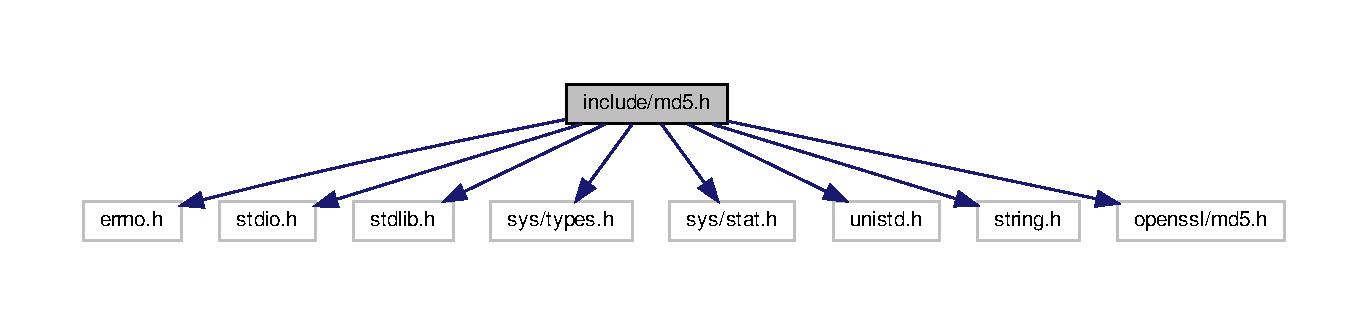
\includegraphics[width=350pt]{md5_8h__incl}
\end{center}
\end{figure}
This graph shows which files directly or indirectly include this file\+:
\nopagebreak
\begin{figure}[H]
\begin{center}
\leavevmode
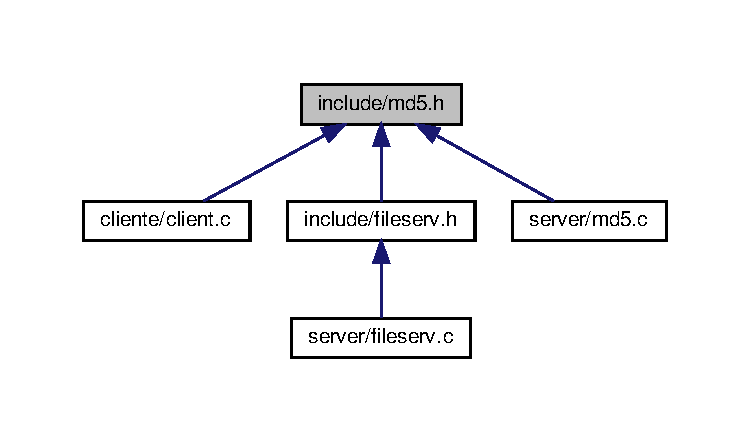
\includegraphics[width=350pt]{md5_8h__dep__incl}
\end{center}
\end{figure}
\subsection*{Macros}
\begin{DoxyCompactItemize}
\item 
\#define \textbf{ B\+U\+F\+F\+S\+I\+ZE}~1024
\end{DoxyCompactItemize}
\subsection*{Functions}
\begin{DoxyCompactItemize}
\item 
char $\ast$ \textbf{ file\+\_\+md5} (char $\ast$, char $\ast$)
\begin{DoxyCompactList}\small\item\em Checksum M\+D5 of filename. \end{DoxyCompactList}\item 
char $\ast$ \textbf{ get\+\_\+md5} (char $\ast$, ssize\+\_\+t, char $\ast$)
\begin{DoxyCompactList}\small\item\em Get the md5 object. \end{DoxyCompactList}\end{DoxyCompactItemize}


\subsection{Macro Definition Documentation}
\mbox{\label{md5_8h_a39912bfe2a55f30e269196f9141d845d}} 
\index{md5.\+h@{md5.\+h}!B\+U\+F\+F\+S\+I\+ZE@{B\+U\+F\+F\+S\+I\+ZE}}
\index{B\+U\+F\+F\+S\+I\+ZE@{B\+U\+F\+F\+S\+I\+ZE}!md5.\+h@{md5.\+h}}
\subsubsection{B\+U\+F\+F\+S\+I\+ZE}
{\footnotesize\ttfamily \#define B\+U\+F\+F\+S\+I\+ZE~1024}



\subsection{Function Documentation}
\mbox{\label{md5_8h_abb8d33df0713fc64b9e32341af87a810}} 
\index{md5.\+h@{md5.\+h}!file\+\_\+md5@{file\+\_\+md5}}
\index{file\+\_\+md5@{file\+\_\+md5}!md5.\+h@{md5.\+h}}
\subsubsection{file\+\_\+md5()}
{\footnotesize\ttfamily char$\ast$ file\+\_\+md5 (\begin{DoxyParamCaption}\item[{char $\ast$}]{filename,  }\item[{char $\ast$}]{md5 }\end{DoxyParamCaption})}



Checksum M\+D5 of filename. 


\begin{DoxyParams}{Parameters}
{\em filename} & \\
\hline
{\em md5} & \\
\hline
\end{DoxyParams}
\begin{DoxyReturn}{Returns}
Formatted string of md5 checksum of file 
\end{DoxyReturn}
\mbox{\label{md5_8h_a882e1f1933e1504e1bb0832a7b226719}} 
\index{md5.\+h@{md5.\+h}!get\+\_\+md5@{get\+\_\+md5}}
\index{get\+\_\+md5@{get\+\_\+md5}!md5.\+h@{md5.\+h}}
\subsubsection{get\+\_\+md5()}
{\footnotesize\ttfamily char$\ast$ get\+\_\+md5 (\begin{DoxyParamCaption}\item[{char $\ast$}]{file\+\_\+path,  }\item[{ssize\+\_\+t}]{end,  }\item[{char $\ast$}]{md5string }\end{DoxyParamCaption})}



Get the md5 object. 


\begin{DoxyParams}{Parameters}
{\em file\+\_\+path} & \\
\hline
{\em end} & \\
\hline
\end{DoxyParams}
\begin{DoxyReturn}{Returns}
char$\ast$ 
\end{DoxyReturn}

\section{include/mq.h File Reference}
\label{mq_8h}\index{include/mq.\+h@{include/mq.\+h}}
{\ttfamily \#include $<$stdio.\+h$>$}\newline
{\ttfamily \#include $<$stdlib.\+h$>$}\newline
{\ttfamily \#include $<$errno.\+h$>$}\newline
{\ttfamily \#include $<$sys/types.\+h$>$}\newline
{\ttfamily \#include $<$sys/ipc.\+h$>$}\newline
{\ttfamily \#include $<$sys/msg.\+h$>$}\newline
{\ttfamily \#include $<$string.\+h$>$}\newline
{\ttfamily \#include $<$unistd.\+h$>$}\newline
Include dependency graph for mq.\+h\+:\nopagebreak
\begin{figure}[H]
\begin{center}
\leavevmode
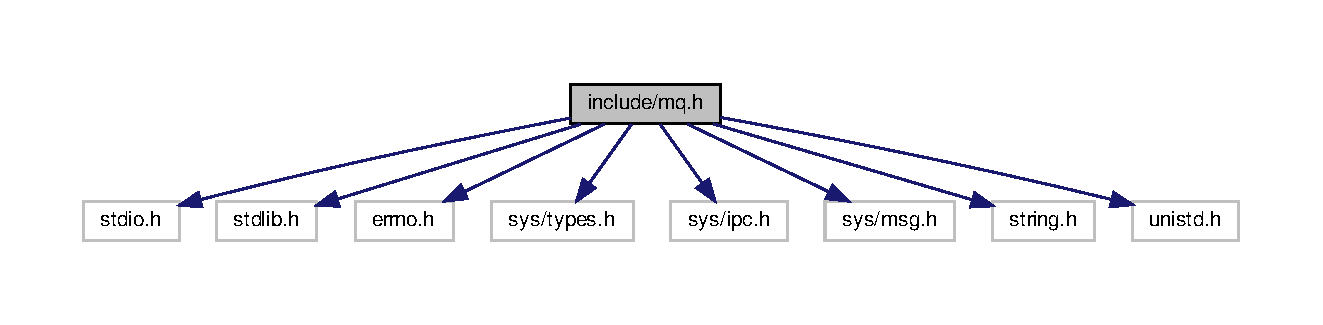
\includegraphics[width=350pt]{mq_8h__incl}
\end{center}
\end{figure}
This graph shows which files directly or indirectly include this file\+:\nopagebreak
\begin{figure}[H]
\begin{center}
\leavevmode
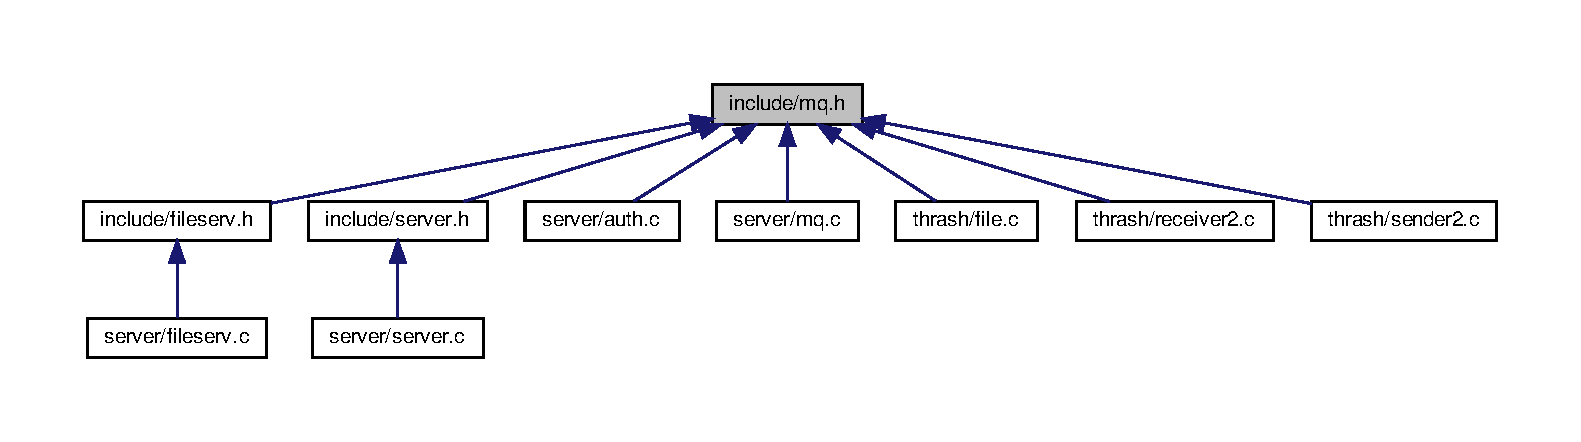
\includegraphics[width=350pt]{mq_8h__dep__incl}
\end{center}
\end{figure}
\subsection*{Data Structures}
\begin{DoxyCompactItemize}
\item 
struct \textbf{ my\+\_\+msgbuf}
\end{DoxyCompactItemize}
\subsection*{Macros}
\begin{DoxyCompactItemize}
\item 
\#define \textbf{ P\+E\+R\+MS}~0644
\item 
\#define \textbf{ B\+U\+F\+F\+S\+I\+ZE}~1024
\end{DoxyCompactItemize}
\subsection*{Functions}
\begin{DoxyCompactItemize}
\item 
int \textbf{ mqid} ()
\begin{DoxyCompactList}\small\item\em Creation of the message queue id. \end{DoxyCompactList}\item 
char $\ast$ \textbf{ rcv\+\_\+msg} (int, char $\ast$, long)
\begin{DoxyCompactList}\small\item\em Wrapper to receive messages from the message queue. \end{DoxyCompactList}\item 
void \textbf{ snd\+\_\+msg} (int, char $\ast$, long)
\begin{DoxyCompactList}\small\item\em Wrapper to send messages to the message queue. \end{DoxyCompactList}\item 
void \textbf{ mq\+\_\+info} (int msqid)
\end{DoxyCompactItemize}


\subsection{Macro Definition Documentation}
\mbox{\label{mq_8h_a39912bfe2a55f30e269196f9141d845d}} 
\index{mq.\+h@{mq.\+h}!B\+U\+F\+F\+S\+I\+ZE@{B\+U\+F\+F\+S\+I\+ZE}}
\index{B\+U\+F\+F\+S\+I\+ZE@{B\+U\+F\+F\+S\+I\+ZE}!mq.\+h@{mq.\+h}}
\subsubsection{B\+U\+F\+F\+S\+I\+ZE}
{\footnotesize\ttfamily \#define B\+U\+F\+F\+S\+I\+ZE~1024}

\mbox{\label{mq_8h_afee0dce2271f56a18b4656548b2de8cc}} 
\index{mq.\+h@{mq.\+h}!P\+E\+R\+MS@{P\+E\+R\+MS}}
\index{P\+E\+R\+MS@{P\+E\+R\+MS}!mq.\+h@{mq.\+h}}
\subsubsection{P\+E\+R\+MS}
{\footnotesize\ttfamily \#define P\+E\+R\+MS~0644}



\subsection{Function Documentation}
\mbox{\label{mq_8h_ad6373ac4d80e0c6198e95bb3a0515ff4}} 
\index{mq.\+h@{mq.\+h}!mq\+\_\+info@{mq\+\_\+info}}
\index{mq\+\_\+info@{mq\+\_\+info}!mq.\+h@{mq.\+h}}
\subsubsection{mq\+\_\+info()}
{\footnotesize\ttfamily void mq\+\_\+info (\begin{DoxyParamCaption}\item[{int}]{msqid }\end{DoxyParamCaption})}

\mbox{\label{mq_8h_aa6a2e92e60754c750bebd73bced350fd}} 
\index{mq.\+h@{mq.\+h}!mqid@{mqid}}
\index{mqid@{mqid}!mq.\+h@{mq.\+h}}
\subsubsection{mqid()}
{\footnotesize\ttfamily int mqid (\begin{DoxyParamCaption}{ }\end{DoxyParamCaption})}



Creation of the message queue id. 

\begin{DoxyReturn}{Returns}
Message queue id 
\end{DoxyReturn}
\mbox{\label{mq_8h_a07daba13b107a4b924dafaa1acf84235}} 
\index{mq.\+h@{mq.\+h}!rcv\+\_\+msg@{rcv\+\_\+msg}}
\index{rcv\+\_\+msg@{rcv\+\_\+msg}!mq.\+h@{mq.\+h}}
\subsubsection{rcv\+\_\+msg()}
{\footnotesize\ttfamily char$\ast$ rcv\+\_\+msg (\begin{DoxyParamCaption}\item[{int}]{msqid,  }\item[{char $\ast$}]{msg,  }\item[{long}]{mtype }\end{DoxyParamCaption})}



Wrapper to receive messages from the message queue. 


\begin{DoxyParams}{Parameters}
{\em msqid} & Message queue ide \\
\hline
{\em msg} & Message received from message queue \\
\hline
{\em mtype} & Message type that identifies the process from which the message should be received \\
\hline
\end{DoxyParams}
\begin{DoxyReturn}{Returns}
String with the message extracted from the message queue 
\end{DoxyReturn}
\mbox{\label{mq_8h_a2e044d5d536ba833380870953724eb03}} 
\index{mq.\+h@{mq.\+h}!snd\+\_\+msg@{snd\+\_\+msg}}
\index{snd\+\_\+msg@{snd\+\_\+msg}!mq.\+h@{mq.\+h}}
\subsubsection{snd\+\_\+msg()}
{\footnotesize\ttfamily void snd\+\_\+msg (\begin{DoxyParamCaption}\item[{int}]{msqid,  }\item[{char $\ast$}]{msg,  }\item[{long}]{mtype }\end{DoxyParamCaption})}



Wrapper to send messages to the message queue. 


\begin{DoxyParams}{Parameters}
{\em msqid} & Message queue ide \\
\hline
{\em msg} & Message received from message queue \\
\hline
{\em mtype} & Message type that identifies the process from which the message should be received \\
\hline
\end{DoxyParams}

\section{include/prompt.h File Reference}
\label{prompt_8h}\index{include/prompt.\+h@{include/prompt.\+h}}
{\ttfamily \#include \char`\"{}common.\+h\char`\"{}}\newline
{\ttfamily \#include $<$stdlib.\+h$>$}\newline
{\ttfamily \#include $<$stdio.\+h$>$}\newline
{\ttfamily \#include $<$string.\+h$>$}\newline
Include dependency graph for prompt.\+h\+:\nopagebreak
\begin{figure}[H]
\begin{center}
\leavevmode
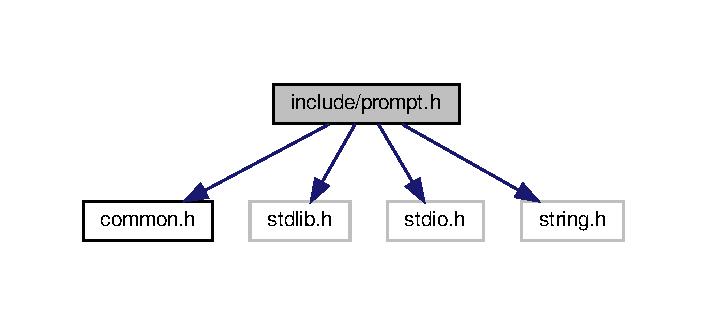
\includegraphics[width=340pt]{prompt_8h__incl}
\end{center}
\end{figure}
This graph shows which files directly or indirectly include this file\+:\nopagebreak
\begin{figure}[H]
\begin{center}
\leavevmode
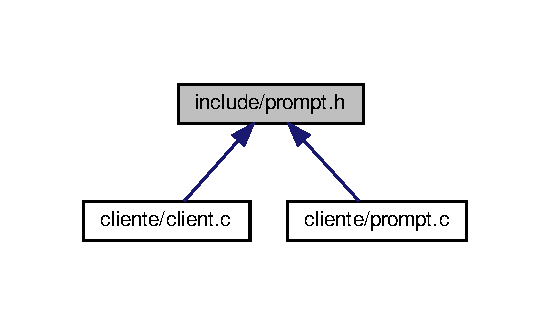
\includegraphics[width=266pt]{prompt_8h__dep__incl}
\end{center}
\end{figure}
\subsection*{Macros}
\begin{DoxyCompactItemize}
\item 
\#define \textbf{ L\+S\+H\+\_\+\+R\+L\+\_\+\+B\+U\+F\+S\+I\+ZE}~1024
\item 
\#define \textbf{ L\+S\+H\+\_\+\+T\+O\+K\+\_\+\+B\+U\+F\+S\+I\+ZE}~64
\item 
\#define \textbf{ L\+S\+H\+\_\+\+T\+O\+K\+\_\+\+D\+E\+L\+IM}~\char`\"{} \textbackslash{}t\textbackslash{}r\textbackslash{}n\textbackslash{}a\char`\"{}
\end{DoxyCompactItemize}
\subsection*{Functions}
\begin{DoxyCompactItemize}
\item 
int \textbf{ argc} (char $\ast$$\ast$)
\begin{DoxyCompactList}\small\item\em Count the number of strings in a string array. \end{DoxyCompactList}\item 
char $\ast$ \textbf{ cmd\+\_\+prompt} (char $\ast$)
\begin{DoxyCompactList}\small\item\em Prompt for the user. \end{DoxyCompactList}\item 
int \textbf{ get\+\_\+cmd} (char $\ast$$\ast$, int)
\begin{DoxyCompactList}\small\item\em Select type of command. \end{DoxyCompactList}\item 
int \textbf{ is\+\_\+exit} (char $\ast$)
\begin{DoxyCompactList}\small\item\em In case of the user has selected the exit command, then exit the prompt. \end{DoxyCompactList}\item 
char $\ast$ \textbf{ read\+\_\+line} (void)
\begin{DoxyCompactList}\small\item\em read line from stdin \end{DoxyCompactList}\item 
char $\ast$$\ast$ \textbf{ split\+\_\+line} (char $\ast$)
\end{DoxyCompactItemize}


\subsection{Macro Definition Documentation}
\mbox{\label{prompt_8h_acffba4e12894ca7015d00aaf3a2354cc}} 
\index{prompt.\+h@{prompt.\+h}!L\+S\+H\+\_\+\+R\+L\+\_\+\+B\+U\+F\+S\+I\+ZE@{L\+S\+H\+\_\+\+R\+L\+\_\+\+B\+U\+F\+S\+I\+ZE}}
\index{L\+S\+H\+\_\+\+R\+L\+\_\+\+B\+U\+F\+S\+I\+ZE@{L\+S\+H\+\_\+\+R\+L\+\_\+\+B\+U\+F\+S\+I\+ZE}!prompt.\+h@{prompt.\+h}}
\subsubsection{L\+S\+H\+\_\+\+R\+L\+\_\+\+B\+U\+F\+S\+I\+ZE}
{\footnotesize\ttfamily \#define L\+S\+H\+\_\+\+R\+L\+\_\+\+B\+U\+F\+S\+I\+ZE~1024}

\mbox{\label{prompt_8h_a5fcc970b08ffddb25a45ab3a875f0905}} 
\index{prompt.\+h@{prompt.\+h}!L\+S\+H\+\_\+\+T\+O\+K\+\_\+\+B\+U\+F\+S\+I\+ZE@{L\+S\+H\+\_\+\+T\+O\+K\+\_\+\+B\+U\+F\+S\+I\+ZE}}
\index{L\+S\+H\+\_\+\+T\+O\+K\+\_\+\+B\+U\+F\+S\+I\+ZE@{L\+S\+H\+\_\+\+T\+O\+K\+\_\+\+B\+U\+F\+S\+I\+ZE}!prompt.\+h@{prompt.\+h}}
\subsubsection{L\+S\+H\+\_\+\+T\+O\+K\+\_\+\+B\+U\+F\+S\+I\+ZE}
{\footnotesize\ttfamily \#define L\+S\+H\+\_\+\+T\+O\+K\+\_\+\+B\+U\+F\+S\+I\+ZE~64}

\mbox{\label{prompt_8h_a27250e82bec993130c5547a5671d61da}} 
\index{prompt.\+h@{prompt.\+h}!L\+S\+H\+\_\+\+T\+O\+K\+\_\+\+D\+E\+L\+IM@{L\+S\+H\+\_\+\+T\+O\+K\+\_\+\+D\+E\+L\+IM}}
\index{L\+S\+H\+\_\+\+T\+O\+K\+\_\+\+D\+E\+L\+IM@{L\+S\+H\+\_\+\+T\+O\+K\+\_\+\+D\+E\+L\+IM}!prompt.\+h@{prompt.\+h}}
\subsubsection{L\+S\+H\+\_\+\+T\+O\+K\+\_\+\+D\+E\+L\+IM}
{\footnotesize\ttfamily \#define L\+S\+H\+\_\+\+T\+O\+K\+\_\+\+D\+E\+L\+IM~\char`\"{} \textbackslash{}t\textbackslash{}r\textbackslash{}n\textbackslash{}a\char`\"{}}



\subsection{Function Documentation}
\mbox{\label{prompt_8h_a6e01607df1054a4c8bcb9604eb191df7}} 
\index{prompt.\+h@{prompt.\+h}!argc@{argc}}
\index{argc@{argc}!prompt.\+h@{prompt.\+h}}
\subsubsection{argc()}
{\footnotesize\ttfamily int argc (\begin{DoxyParamCaption}\item[{char $\ast$$\ast$}]{n }\end{DoxyParamCaption})}



Count the number of strings in a string array. 


\begin{DoxyParams}{Parameters}
{\em n} & array of strings \\
\hline
\end{DoxyParams}
\begin{DoxyReturn}{Returns}
number of strings 
\end{DoxyReturn}
\mbox{\label{prompt_8h_ae3a964495cbc932650f78912457f90af}} 
\index{prompt.\+h@{prompt.\+h}!cmd\+\_\+prompt@{cmd\+\_\+prompt}}
\index{cmd\+\_\+prompt@{cmd\+\_\+prompt}!prompt.\+h@{prompt.\+h}}
\subsubsection{cmd\+\_\+prompt()}
{\footnotesize\ttfamily char$\ast$ cmd\+\_\+prompt (\begin{DoxyParamCaption}\item[{char $\ast$}]{str\+\_\+to\+\_\+server }\end{DoxyParamCaption})}



Prompt for the user. 

All possibilities are contemplated to achieve robust behavior of the function. This may make it look a bit complex but it is properly documented for understanding the code. 
\begin{DoxyParams}{Parameters}
{\em str\+\_\+to\+\_\+server} & String to be sent to the server \\
\hline
\end{DoxyParams}
\begin{DoxyReturn}{Returns}
pointer to string  
\end{DoxyReturn}
Start of the prompt, it is kept in a do-\/while loop until the user enters a valid command.\mbox{\label{prompt_8h_ae8fac212768cd6eac01f65cf151b3a43}} 
\index{prompt.\+h@{prompt.\+h}!get\+\_\+cmd@{get\+\_\+cmd}}
\index{get\+\_\+cmd@{get\+\_\+cmd}!prompt.\+h@{prompt.\+h}}
\subsubsection{get\+\_\+cmd()}
{\footnotesize\ttfamily int get\+\_\+cmd (\begin{DoxyParamCaption}\item[{char $\ast$$\ast$}]{args,  }\item[{int}]{n\+\_\+args }\end{DoxyParamCaption})}



Select type of command. 

In case the first argument is any of the valid commands, the function will return an int greater than or equal to zero. If not it will return a negative int. 
\begin{DoxyParams}{Parameters}
{\em args} & Array of tokenized strings coming from user prompt \\
\hline
{\em n\+\_\+args} & Number of elements of array args \\
\hline
\end{DoxyParams}
\begin{DoxyReturn}{Returns}
int 
\end{DoxyReturn}
\mbox{\label{prompt_8h_aaae547d76bf7da0f67987d3f2f2d537f}} 
\index{prompt.\+h@{prompt.\+h}!is\+\_\+exit@{is\+\_\+exit}}
\index{is\+\_\+exit@{is\+\_\+exit}!prompt.\+h@{prompt.\+h}}
\subsubsection{is\+\_\+exit()}
{\footnotesize\ttfamily int is\+\_\+exit (\begin{DoxyParamCaption}\item[{char $\ast$}]{str }\end{DoxyParamCaption})}



In case of the user has selected the exit command, then exit the prompt. 


\begin{DoxyParams}{Parameters}
{\em str} & str\+\_\+to\+\_\+server \\
\hline
\end{DoxyParams}
\begin{DoxyReturn}{Returns}
int 
\end{DoxyReturn}
\mbox{\label{prompt_8h_ac14a4d3d27ec36419b82f72342be3a65}} 
\index{prompt.\+h@{prompt.\+h}!read\+\_\+line@{read\+\_\+line}}
\index{read\+\_\+line@{read\+\_\+line}!prompt.\+h@{prompt.\+h}}
\subsubsection{read\+\_\+line()}
{\footnotesize\ttfamily char$\ast$ read\+\_\+line (\begin{DoxyParamCaption}\item[{void}]{ }\end{DoxyParamCaption})}



read line from stdin 

\begin{DoxyReturn}{Returns}
char $\ast$ with the line 
\end{DoxyReturn}
\mbox{\label{prompt_8h_ae3787b54051a7b49115846f09e9716c9}} 
\index{prompt.\+h@{prompt.\+h}!split\+\_\+line@{split\+\_\+line}}
\index{split\+\_\+line@{split\+\_\+line}!prompt.\+h@{prompt.\+h}}
\subsubsection{split\+\_\+line()}
{\footnotesize\ttfamily char$\ast$$\ast$ split\+\_\+line (\begin{DoxyParamCaption}\item[{char $\ast$}]{line }\end{DoxyParamCaption})}


\begin{DoxyParams}{Parameters}
{\em line} & \\
\hline
\end{DoxyParams}
\begin{DoxyReturn}{Returns}
char$\ast$$\ast$ 
\end{DoxyReturn}

\section{include/server.h File Reference}
\label{server_8h}\index{include/server.\+h@{include/server.\+h}}
{\ttfamily \#include \char`\"{}socket.\+h\char`\"{}}\newline
{\ttfamily \#include \char`\"{}mq.\+h\char`\"{}}\newline
{\ttfamily \#include \char`\"{}common.\+h\char`\"{}}\newline
{\ttfamily \#include $<$sys/types.\+h$>$}\newline
{\ttfamily \#include $<$sys/wait.\+h$>$}\newline
Include dependency graph for server.\+h\+:
\nopagebreak
\begin{figure}[H]
\begin{center}
\leavevmode
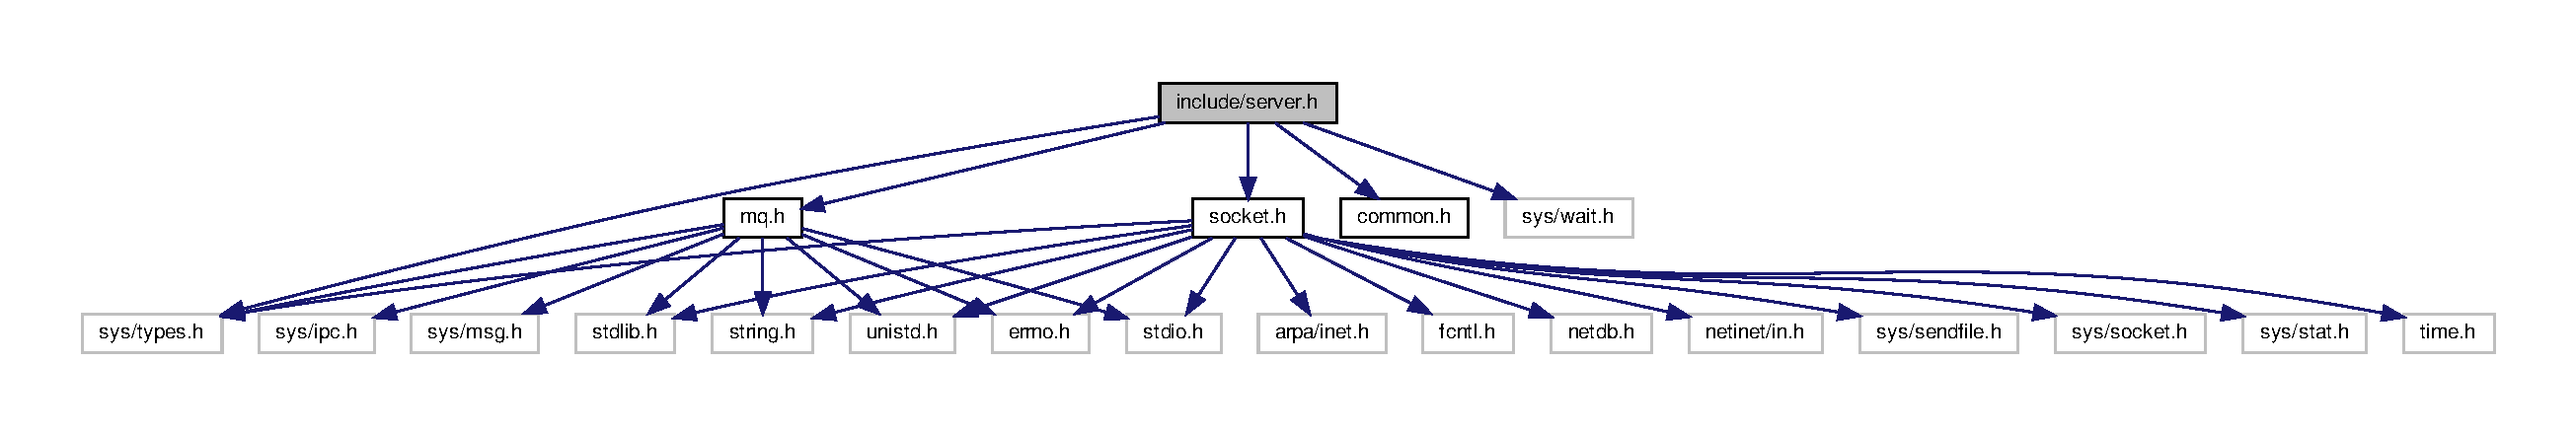
\includegraphics[width=350pt]{server_8h__incl}
\end{center}
\end{figure}
This graph shows which files directly or indirectly include this file\+:
\nopagebreak
\begin{figure}[H]
\begin{center}
\leavevmode
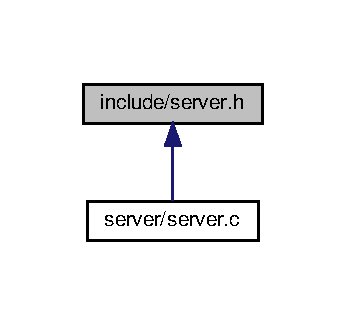
\includegraphics[width=166pt]{server_8h__dep__incl}
\end{center}
\end{figure}
\subsection*{Functions}
\begin{DoxyCompactItemize}
\item 
long \textbf{ get\+\_\+1st\+\_\+char} (char $\ast$)
\begin{DoxyCompactList}\small\item\em Get the 1st char of str. \end{DoxyCompactList}\item 
long \textbf{ cmd\+\_\+handler} (char $\ast$, char $\ast$)
\begin{DoxyCompactList}\small\item\em Decode the str that comes from the client and then be forwarded to A\+UT or F\+LS as appropriate. \end{DoxyCompactList}\item 
void \textbf{ login\+\_\+handler} (int, int)
\begin{DoxyCompactList}\small\item\em Login handler between auth and server. \end{DoxyCompactList}\item 
void \textbf{ rcv\+\_\+cmd} (int, int)
\begin{DoxyCompactList}\small\item\em Login handler between [A\+UT] and [S\+RV]. \end{DoxyCompactList}\end{DoxyCompactItemize}


\subsection{Function Documentation}
\mbox{\label{server_8h_a4199c4fe35b146a5a21818e16572ce17}} 
\index{server.\+h@{server.\+h}!cmd\+\_\+handler@{cmd\+\_\+handler}}
\index{cmd\+\_\+handler@{cmd\+\_\+handler}!server.\+h@{server.\+h}}
\subsubsection{cmd\+\_\+handler()}
{\footnotesize\ttfamily long cmd\+\_\+handler (\begin{DoxyParamCaption}\item[{char $\ast$}]{cmd,  }\item[{char $\ast$}]{msg }\end{DoxyParamCaption})}



Decode the str that comes from the client and then be forwarded to A\+UT or F\+LS as appropriate. 


\begin{DoxyParams}{Parameters}
{\em cmd} & \\
\hline
{\em msg} & \\
\hline
\end{DoxyParams}
\begin{DoxyReturn}{Returns}
long m\+\_\+type 
\end{DoxyReturn}
\mbox{\label{server_8h_a293029f59f0b388380b8491d52f8e867}} 
\index{server.\+h@{server.\+h}!get\+\_\+1st\+\_\+char@{get\+\_\+1st\+\_\+char}}
\index{get\+\_\+1st\+\_\+char@{get\+\_\+1st\+\_\+char}!server.\+h@{server.\+h}}
\subsubsection{get\+\_\+1st\+\_\+char()}
{\footnotesize\ttfamily long get\+\_\+1st\+\_\+char (\begin{DoxyParamCaption}\item[{char $\ast$}]{str }\end{DoxyParamCaption})}



Get the 1st char of str. 


\begin{DoxyParams}{Parameters}
{\em str} & \\
\hline
\end{DoxyParams}
\begin{DoxyReturn}{Returns}
long 
\end{DoxyReturn}
\mbox{\label{server_8h_ac8306e493111b55b1bcf59a26e9a45b6}} 
\index{server.\+h@{server.\+h}!login\+\_\+handler@{login\+\_\+handler}}
\index{login\+\_\+handler@{login\+\_\+handler}!server.\+h@{server.\+h}}
\subsubsection{login\+\_\+handler()}
{\footnotesize\ttfamily void login\+\_\+handler (\begin{DoxyParamCaption}\item[{int}]{sockfd,  }\item[{int}]{msqid }\end{DoxyParamCaption})}



Login handler between auth and server. 


\begin{DoxyParams}{Parameters}
{\em sockfd} & \\
\hline
{\em msqid} & \\
\hline
\end{DoxyParams}
\mbox{\label{server_8h_a9e01af92870c6e74d3b55dd7aab75cb7}} 
\index{server.\+h@{server.\+h}!rcv\+\_\+cmd@{rcv\+\_\+cmd}}
\index{rcv\+\_\+cmd@{rcv\+\_\+cmd}!server.\+h@{server.\+h}}
\subsubsection{rcv\+\_\+cmd()}
{\footnotesize\ttfamily void rcv\+\_\+cmd (\begin{DoxyParamCaption}\item[{int}]{sockfd,  }\item[{int}]{msqid }\end{DoxyParamCaption})}



Login handler between [A\+UT] and [S\+RV]. 


\begin{DoxyParams}{Parameters}
{\em sockfd} & \\
\hline
{\em msqid} & \\
\hline
\end{DoxyParams}

\input{include_2socket_8h}
\input{thrash_2socket_8h}
\section{R\+E\+A\+D\+M\+E.\+md File Reference}
\label{_r_e_a_d_m_e_8md}\index{R\+E\+A\+D\+M\+E.\+md@{R\+E\+A\+D\+M\+E.\+md}}

\section{server/auth.c File Reference}
\label{auth_8c}\index{server/auth.\+c@{server/auth.\+c}}
{\ttfamily \#include \char`\"{}auth.\+h\char`\"{}}\newline
{\ttfamily \#include \char`\"{}mq.\+h\char`\"{}}\newline
Include dependency graph for auth.\+c\+:\nopagebreak
\begin{figure}[H]
\begin{center}
\leavevmode
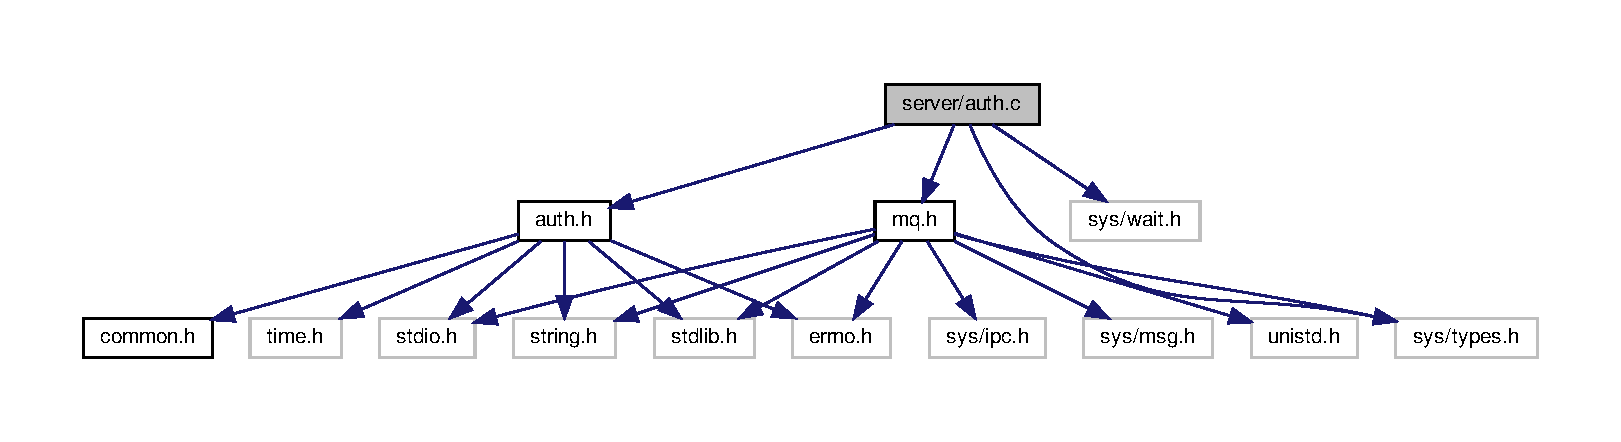
\includegraphics[width=350pt]{auth_8c__incl}
\end{center}
\end{figure}
\subsection*{Functions}
\begin{DoxyCompactItemize}
\item 
int \textbf{ main} (void)
\item 
void \textbf{ last\+\_\+connect} (char $\ast$\textbf{ user})
\begin{DoxyCompactList}\small\item\em Registers the date of the login of a user saving the value in the database. \end{DoxyCompactList}\item 
void \textbf{ increase\+\_\+block} (char $\ast$\textbf{ user})
\begin{DoxyCompactList}\small\item\em Increase number of blocks according to user. \end{DoxyCompactList}\item 
int \textbf{ check\+\_\+block} (char $\ast$\textbf{ user})
\begin{DoxyCompactList}\small\item\em Check the number of user blocks. \end{DoxyCompactList}\item 
int \textbf{ get\+\_\+status} (char $\ast$userpass, char $\ast$\textbf{ user})
\begin{DoxyCompactList}\small\item\em Get the status of check userpass. \end{DoxyCompactList}\item 
char $\ast$ \textbf{ login\+\_\+handler} (int msqid, char $\ast$\textbf{ user})
\begin{DoxyCompactList}\small\item\em Login handler between [A\+UT] and [S\+RV]. \end{DoxyCompactList}\item 
char $\ast$ \textbf{ get\+\_\+pass} (char $\ast$str)
\begin{DoxyCompactList}\small\item\em Returns the pass substr of str. \end{DoxyCompactList}\item 
int \textbf{ cmd\+\_\+handler} (int msqid, char $\ast$\textbf{ user})
\begin{DoxyCompactList}\small\item\em Login handler between [A\+UT] and [S\+RV]. \end{DoxyCompactList}\item 
char $\ast$ \textbf{ list\+\_\+users} (char $\ast$str\+Users)
\begin{DoxyCompactList}\small\item\em List users in DB. \end{DoxyCompactList}\item 
void \textbf{ load\+\_\+db} (void)
\begin{DoxyCompactList}\small\item\em Load users to DB from C\+SV file. \end{DoxyCompactList}\item 
void \textbf{ change\+\_\+pass} (char $\ast$\textbf{ user}, char $\ast$pass)
\begin{DoxyCompactList}\small\item\em Change user pass in DB. \end{DoxyCompactList}\item 
void \textbf{ save\+\_\+db} ()
\begin{DoxyCompactList}\small\item\em Save DB changes in C\+SV file. \end{DoxyCompactList}\item 
int \textbf{ check\+\_\+pass} (char $\ast$\textbf{ user}, char $\ast$pass)
\begin{DoxyCompactList}\small\item\em Change user pass in DB. \end{DoxyCompactList}\end{DoxyCompactItemize}


\subsection{Function Documentation}
\mbox{\label{auth_8c_a94e83fe1538f3e714f97775e42b00843}} 
\index{auth.\+c@{auth.\+c}!change\+\_\+pass@{change\+\_\+pass}}
\index{change\+\_\+pass@{change\+\_\+pass}!auth.\+c@{auth.\+c}}
\subsubsection{change\+\_\+pass()}
{\footnotesize\ttfamily void change\+\_\+pass (\begin{DoxyParamCaption}\item[{char $\ast$}]{user,  }\item[{char $\ast$}]{pass }\end{DoxyParamCaption})}



Change user pass in DB. 


\begin{DoxyParams}{Parameters}
{\em user} & \\
\hline
{\em pass} & \\
\hline
\end{DoxyParams}
\mbox{\label{auth_8c_a4ab3ea5859f626a770d03db44f7a41aa}} 
\index{auth.\+c@{auth.\+c}!check\+\_\+block@{check\+\_\+block}}
\index{check\+\_\+block@{check\+\_\+block}!auth.\+c@{auth.\+c}}
\subsubsection{check\+\_\+block()}
{\footnotesize\ttfamily int check\+\_\+block (\begin{DoxyParamCaption}\item[{char $\ast$}]{user }\end{DoxyParamCaption})}



Check the number of user blocks. 


\begin{DoxyParams}{Parameters}
{\em user} & \\
\hline
\end{DoxyParams}
\begin{DoxyReturn}{Returns}
int 1 if user have 3 or more blocks. else 0. 
\end{DoxyReturn}
\mbox{\label{auth_8c_a3db4ab1fb0409a005f819caa6623865d}} 
\index{auth.\+c@{auth.\+c}!check\+\_\+pass@{check\+\_\+pass}}
\index{check\+\_\+pass@{check\+\_\+pass}!auth.\+c@{auth.\+c}}
\subsubsection{check\+\_\+pass()}
{\footnotesize\ttfamily int check\+\_\+pass (\begin{DoxyParamCaption}\item[{char $\ast$}]{user,  }\item[{char $\ast$}]{pass }\end{DoxyParamCaption})}



Change user pass in DB. 


\begin{DoxyParams}{Parameters}
{\em user} & \\
\hline
{\em pass} & \\
\hline
\end{DoxyParams}
\mbox{\label{auth_8c_a9aad4fc4e148f0c94e1c891951a824aa}} 
\index{auth.\+c@{auth.\+c}!cmd\+\_\+handler@{cmd\+\_\+handler}}
\index{cmd\+\_\+handler@{cmd\+\_\+handler}!auth.\+c@{auth.\+c}}
\subsubsection{cmd\+\_\+handler()}
{\footnotesize\ttfamily int cmd\+\_\+handler (\begin{DoxyParamCaption}\item[{int}]{msqid,  }\item[{char $\ast$}]{user }\end{DoxyParamCaption})}



Login handler between [A\+UT] and [S\+RV]. 


\begin{DoxyParams}{Parameters}
{\em msqid} & \\
\hline
\end{DoxyParams}
\mbox{\label{auth_8c_a2e12b8307c78eca77ba679c218546ea9}} 
\index{auth.\+c@{auth.\+c}!get\+\_\+pass@{get\+\_\+pass}}
\index{get\+\_\+pass@{get\+\_\+pass}!auth.\+c@{auth.\+c}}
\subsubsection{get\+\_\+pass()}
{\footnotesize\ttfamily char$\ast$ get\+\_\+pass (\begin{DoxyParamCaption}\item[{char $\ast$}]{str }\end{DoxyParamCaption})}



Returns the pass substr of str. 


\begin{DoxyParams}{Parameters}
{\em str} & \\
\hline
\end{DoxyParams}
\begin{DoxyReturn}{Returns}
char$\ast$ 
\end{DoxyReturn}
\mbox{\label{auth_8c_afb230134b9c54844c1d46a4aff308423}} 
\index{auth.\+c@{auth.\+c}!get\+\_\+status@{get\+\_\+status}}
\index{get\+\_\+status@{get\+\_\+status}!auth.\+c@{auth.\+c}}
\subsubsection{get\+\_\+status()}
{\footnotesize\ttfamily int get\+\_\+status (\begin{DoxyParamCaption}\item[{char $\ast$}]{userpass,  }\item[{char $\ast$}]{user }\end{DoxyParamCaption})}



Get the status of check userpass. 


\begin{DoxyParams}{Parameters}
{\em userpass} & \\
\hline
\end{DoxyParams}
\begin{DoxyReturn}{Returns}
int 1\+: user and pass correct. 0\+: pass wrong. -\/1\+: user wrong. -\/2\+: user blocked. 
\end{DoxyReturn}
\mbox{\label{auth_8c_a5477481a6cf3be8d1fea01a8d35ceff2}} 
\index{auth.\+c@{auth.\+c}!increase\+\_\+block@{increase\+\_\+block}}
\index{increase\+\_\+block@{increase\+\_\+block}!auth.\+c@{auth.\+c}}
\subsubsection{increase\+\_\+block()}
{\footnotesize\ttfamily void increase\+\_\+block (\begin{DoxyParamCaption}\item[{char $\ast$}]{user }\end{DoxyParamCaption})}



Increase number of blocks according to user. 


\begin{DoxyParams}{Parameters}
{\em user} & \\
\hline
\end{DoxyParams}
\mbox{\label{auth_8c_adedb2d3fe2edbbc0dc8873423f20a23b}} 
\index{auth.\+c@{auth.\+c}!last\+\_\+connect@{last\+\_\+connect}}
\index{last\+\_\+connect@{last\+\_\+connect}!auth.\+c@{auth.\+c}}
\subsubsection{last\+\_\+connect()}
{\footnotesize\ttfamily void last\+\_\+connect (\begin{DoxyParamCaption}\item[{char $\ast$}]{user }\end{DoxyParamCaption})}



Registers the date of the login of a user saving the value in the database. 


\begin{DoxyParams}{Parameters}
{\em user} & \\
\hline
\end{DoxyParams}
\mbox{\label{auth_8c_a057d702fc9dbc94e59ee567c7d9f0a6e}} 
\index{auth.\+c@{auth.\+c}!list\+\_\+users@{list\+\_\+users}}
\index{list\+\_\+users@{list\+\_\+users}!auth.\+c@{auth.\+c}}
\subsubsection{list\+\_\+users()}
{\footnotesize\ttfamily char$\ast$ list\+\_\+users (\begin{DoxyParamCaption}\item[{char $\ast$}]{str\+Users }\end{DoxyParamCaption})}



List users in DB. 


\begin{DoxyParams}{Parameters}
{\em str\+Users} & \\
\hline
\end{DoxyParams}
\begin{DoxyReturn}{Returns}
char$\ast$ with users information. 
\end{DoxyReturn}
\mbox{\label{auth_8c_aca138a298c612a14d6fb2c16672f8c87}} 
\index{auth.\+c@{auth.\+c}!load\+\_\+db@{load\+\_\+db}}
\index{load\+\_\+db@{load\+\_\+db}!auth.\+c@{auth.\+c}}
\subsubsection{load\+\_\+db()}
{\footnotesize\ttfamily void load\+\_\+db (\begin{DoxyParamCaption}\item[{void}]{ }\end{DoxyParamCaption})}



Load users to DB from C\+SV file. 

\mbox{\label{auth_8c_adac4679e3a9744c45353d68b35bd1aba}} 
\index{auth.\+c@{auth.\+c}!login\+\_\+handler@{login\+\_\+handler}}
\index{login\+\_\+handler@{login\+\_\+handler}!auth.\+c@{auth.\+c}}
\subsubsection{login\+\_\+handler()}
{\footnotesize\ttfamily char$\ast$ login\+\_\+handler (\begin{DoxyParamCaption}\item[{int}]{msqid,  }\item[{char $\ast$}]{user }\end{DoxyParamCaption})}



Login handler between [A\+UT] and [S\+RV]. 


\begin{DoxyParams}{Parameters}
{\em msqid} & \\
\hline
\end{DoxyParams}
\mbox{\label{auth_8c_a840291bc02cba5474a4cb46a9b9566fe}} 
\index{auth.\+c@{auth.\+c}!main@{main}}
\index{main@{main}!auth.\+c@{auth.\+c}}
\subsubsection{main()}
{\footnotesize\ttfamily int main (\begin{DoxyParamCaption}\item[{void}]{ }\end{DoxyParamCaption})}

\mbox{\label{auth_8c_afeb75f74451938ff9dc7617224f6fe3f}} 
\index{auth.\+c@{auth.\+c}!save\+\_\+db@{save\+\_\+db}}
\index{save\+\_\+db@{save\+\_\+db}!auth.\+c@{auth.\+c}}
\subsubsection{save\+\_\+db()}
{\footnotesize\ttfamily void save\+\_\+db (\begin{DoxyParamCaption}\item[{void}]{ }\end{DoxyParamCaption})}



Save DB changes in C\+SV file. 


\section{server/fileserv.c File Reference}
\label{fileserv_8c}\index{server/fileserv.\+c@{server/fileserv.\+c}}
{\ttfamily \#include \char`\"{}fileserv.\+h\char`\"{}}\newline
Include dependency graph for fileserv.\+c\+:\nopagebreak
\begin{figure}[H]
\begin{center}
\leavevmode
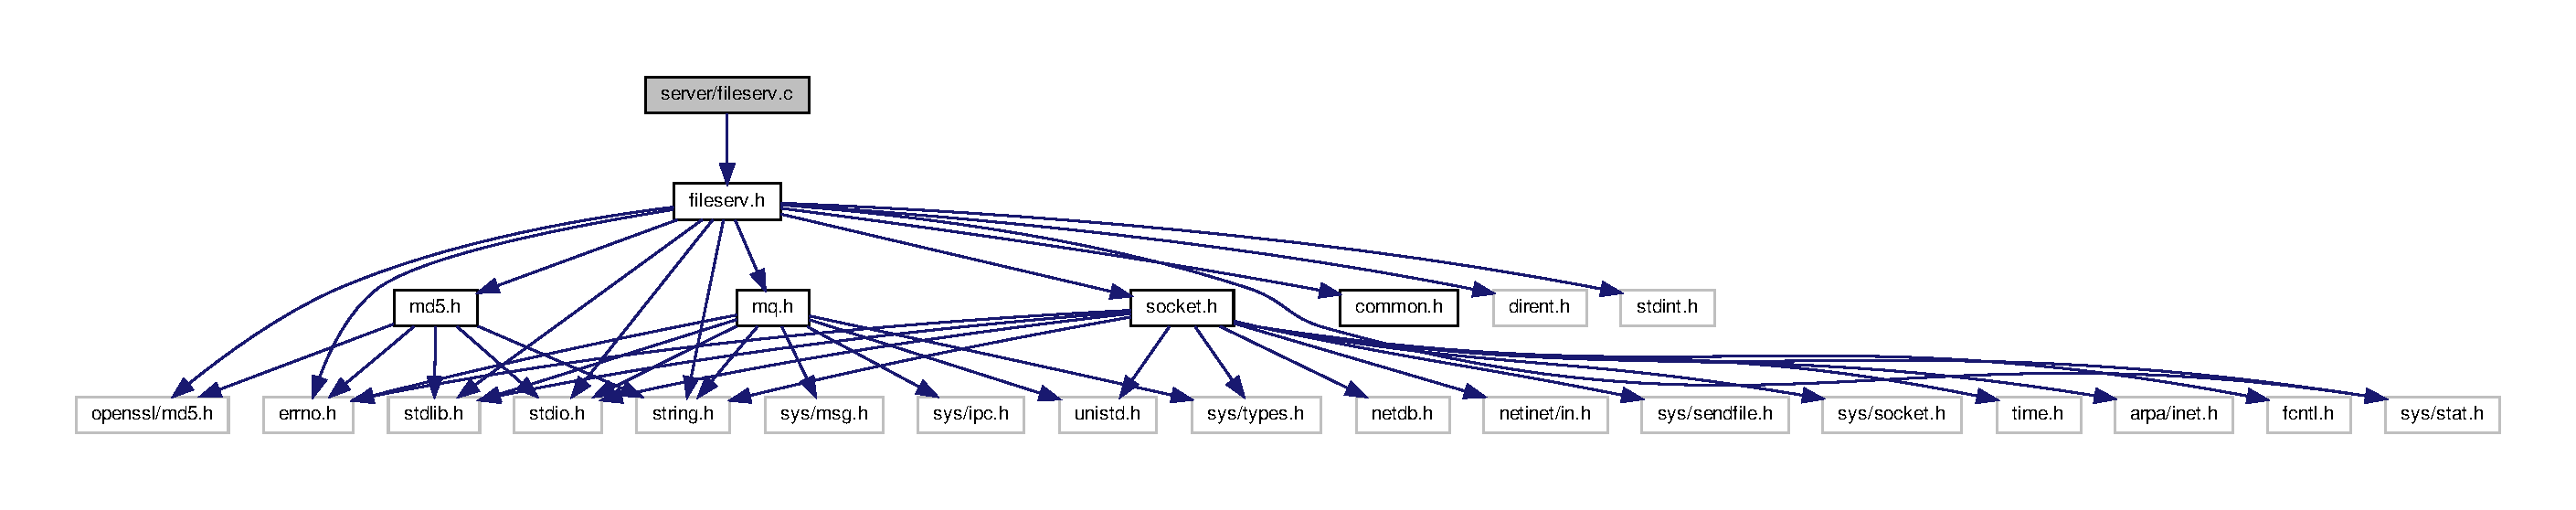
\includegraphics[width=350pt]{fileserv_8c__incl}
\end{center}
\end{figure}
\subsection*{Functions}
\begin{DoxyCompactItemize}
\item 
int \textbf{ main} (void)
\item 
char $\ast$ \textbf{ readable\+\_\+fs} (long int size, char $\ast$buf)
\begin{DoxyCompactList}\small\item\em Parser that returns in human-\/readable format the size of a file. \end{DoxyCompactList}\item 
char $\ast$ \textbf{ files\+\_\+info} (char $\ast$files\+Info)
\begin{DoxyCompactList}\small\item\em Collection of the required information for each file in a specific folder. \end{DoxyCompactList}\item 
int \textbf{ is\+\_\+valid\+\_\+file} (char $\ast$str)
\begin{DoxyCompactList}\small\item\em Iterates through all the items in the folder until find the required file. \end{DoxyCompactList}\item 
int \textbf{ check\+\_\+file} (char $\ast$str, char $\ast$file)
\begin{DoxyCompactList}\small\item\em Checks the existence of the image in the folder img. \end{DoxyCompactList}\item 
void \textbf{ transfer\+\_\+fs} (char $\ast$file)
\begin{DoxyCompactList}\small\item\em Sockets are created and the file is sent to the client. \end{DoxyCompactList}\item 
int \textbf{ cmd\+\_\+handler} (int msqid)
\begin{DoxyCompactList}\small\item\em Command handler. \end{DoxyCompactList}\end{DoxyCompactItemize}


\subsection{Function Documentation}
\mbox{\label{fileserv_8c_a934e48b50634987f1069e535f4f9753a}} 
\index{fileserv.\+c@{fileserv.\+c}!check\+\_\+file@{check\+\_\+file}}
\index{check\+\_\+file@{check\+\_\+file}!fileserv.\+c@{fileserv.\+c}}
\subsubsection{check\+\_\+file()}
{\footnotesize\ttfamily int check\+\_\+file (\begin{DoxyParamCaption}\item[{char $\ast$}]{str,  }\item[{char $\ast$}]{file }\end{DoxyParamCaption})}



Checks the existence of the image in the folder img. 


\begin{DoxyParams}{Parameters}
{\em str} & string to client \\
\hline
{\em file} & filename \\
\hline
\end{DoxyParams}
\begin{DoxyReturn}{Returns}
int tf 
\end{DoxyReturn}
\mbox{\label{fileserv_8c_a975d9337db509c0204b110f51d723160}} 
\index{fileserv.\+c@{fileserv.\+c}!cmd\+\_\+handler@{cmd\+\_\+handler}}
\index{cmd\+\_\+handler@{cmd\+\_\+handler}!fileserv.\+c@{fileserv.\+c}}
\subsubsection{cmd\+\_\+handler()}
{\footnotesize\ttfamily int cmd\+\_\+handler (\begin{DoxyParamCaption}\item[{int}]{msqid }\end{DoxyParamCaption})}



Command handler. 


\begin{DoxyParams}{Parameters}
{\em msqid} & \\
\hline
\end{DoxyParams}
\begin{DoxyReturn}{Returns}
int exit 
\end{DoxyReturn}
\mbox{\label{fileserv_8c_a28f9a6d37e4dbc8b5bf5fad1025285e3}} 
\index{fileserv.\+c@{fileserv.\+c}!files\+\_\+info@{files\+\_\+info}}
\index{files\+\_\+info@{files\+\_\+info}!fileserv.\+c@{fileserv.\+c}}
\subsubsection{files\+\_\+info()}
{\footnotesize\ttfamily char$\ast$ files\+\_\+info (\begin{DoxyParamCaption}\item[{char $\ast$}]{files\+Info }\end{DoxyParamCaption})}



Collection of the required information for each file in a specific folder. 


\begin{DoxyParams}{Parameters}
{\em files\+Info} & \\
\hline
\end{DoxyParams}
\begin{DoxyReturn}{Returns}
Formatted string ready to be printed or sent 
\end{DoxyReturn}
\mbox{\label{fileserv_8c_aaac1f10c2cd0525412fb92d9279b0670}} 
\index{fileserv.\+c@{fileserv.\+c}!is\+\_\+valid\+\_\+file@{is\+\_\+valid\+\_\+file}}
\index{is\+\_\+valid\+\_\+file@{is\+\_\+valid\+\_\+file}!fileserv.\+c@{fileserv.\+c}}
\subsubsection{is\+\_\+valid\+\_\+file()}
{\footnotesize\ttfamily int is\+\_\+valid\+\_\+file (\begin{DoxyParamCaption}\item[{char $\ast$}]{str }\end{DoxyParamCaption})}



Iterates through all the items in the folder until find the required file. 


\begin{DoxyParams}{Parameters}
{\em str} & filename \\
\hline
\end{DoxyParams}
\begin{DoxyReturn}{Returns}
int 
\end{DoxyReturn}
\mbox{\label{fileserv_8c_a840291bc02cba5474a4cb46a9b9566fe}} 
\index{fileserv.\+c@{fileserv.\+c}!main@{main}}
\index{main@{main}!fileserv.\+c@{fileserv.\+c}}
\subsubsection{main()}
{\footnotesize\ttfamily int main (\begin{DoxyParamCaption}\item[{void}]{ }\end{DoxyParamCaption})}

\mbox{\label{fileserv_8c_acb8985a720cf17b68e99872ba793f2cc}} 
\index{fileserv.\+c@{fileserv.\+c}!readable\+\_\+fs@{readable\+\_\+fs}}
\index{readable\+\_\+fs@{readable\+\_\+fs}!fileserv.\+c@{fileserv.\+c}}
\subsubsection{readable\+\_\+fs()}
{\footnotesize\ttfamily char$\ast$ readable\+\_\+fs (\begin{DoxyParamCaption}\item[{long int}]{size,  }\item[{char $\ast$}]{buf }\end{DoxyParamCaption})}



Parser that returns in human-\/readable format the size of a file. 


\begin{DoxyParams}{Parameters}
{\em size} & in bytes from file \\
\hline
{\em buf} & string \\
\hline
\end{DoxyParams}
\begin{DoxyReturn}{Returns}
Formatted string what contains human-\/readable size of file. 
\end{DoxyReturn}
\mbox{\label{fileserv_8c_a5ea0687811fad6f1c67348a52ec2bb7a}} 
\index{fileserv.\+c@{fileserv.\+c}!transfer\+\_\+fs@{transfer\+\_\+fs}}
\index{transfer\+\_\+fs@{transfer\+\_\+fs}!fileserv.\+c@{fileserv.\+c}}
\subsubsection{transfer\+\_\+fs()}
{\footnotesize\ttfamily void transfer\+\_\+fs (\begin{DoxyParamCaption}\item[{char $\ast$}]{file }\end{DoxyParamCaption})}



Sockets are created and the file is sent to the client. 


\begin{DoxyParams}{Parameters}
{\em file} & \\
\hline
\end{DoxyParams}

\section{server/md5.c File Reference}
\label{md5_8c}\index{server/md5.\+c@{server/md5.\+c}}
{\ttfamily \#include \char`\"{}md5.\+h\char`\"{}}\newline
Include dependency graph for md5.\+c\+:\nopagebreak
\begin{figure}[H]
\begin{center}
\leavevmode
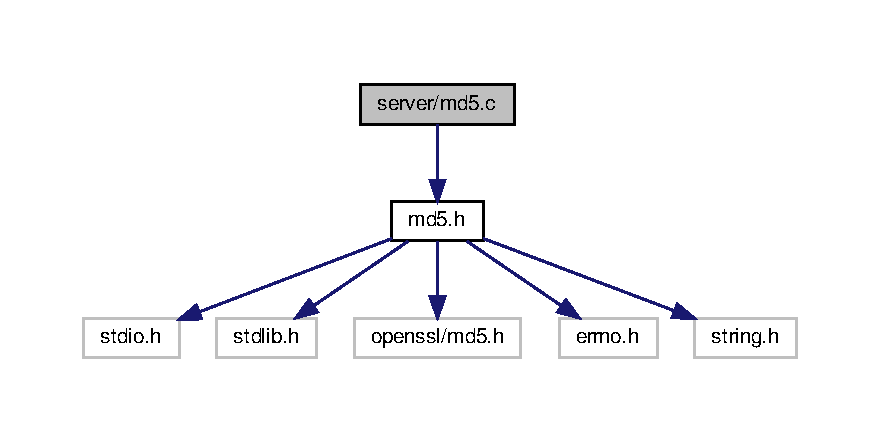
\includegraphics[width=350pt]{md5_8c__incl}
\end{center}
\end{figure}
\subsection*{Macros}
\begin{DoxyCompactItemize}
\item 
\#define \textbf{ B\+U\+F\+F\+S\+I\+ZE}~1024
\end{DoxyCompactItemize}
\subsection*{Functions}
\begin{DoxyCompactItemize}
\item 
char $\ast$ \textbf{ file\+\_\+md5} (char $\ast$filename, char $\ast$md5)
\begin{DoxyCompactList}\small\item\em Checksum M\+D5 of filename. \end{DoxyCompactList}\end{DoxyCompactItemize}


\subsection{Macro Definition Documentation}
\mbox{\label{md5_8c_a39912bfe2a55f30e269196f9141d845d}} 
\index{md5.\+c@{md5.\+c}!B\+U\+F\+F\+S\+I\+ZE@{B\+U\+F\+F\+S\+I\+ZE}}
\index{B\+U\+F\+F\+S\+I\+ZE@{B\+U\+F\+F\+S\+I\+ZE}!md5.\+c@{md5.\+c}}
\subsubsection{B\+U\+F\+F\+S\+I\+ZE}
{\footnotesize\ttfamily \#define B\+U\+F\+F\+S\+I\+ZE~1024}



\subsection{Function Documentation}
\mbox{\label{md5_8c_adaa982699055a63eb33d040e7d13f965}} 
\index{md5.\+c@{md5.\+c}!file\+\_\+md5@{file\+\_\+md5}}
\index{file\+\_\+md5@{file\+\_\+md5}!md5.\+c@{md5.\+c}}
\subsubsection{file\+\_\+md5()}
{\footnotesize\ttfamily char$\ast$ file\+\_\+md5 (\begin{DoxyParamCaption}\item[{char $\ast$}]{filename,  }\item[{char $\ast$}]{md5 }\end{DoxyParamCaption})}



Checksum M\+D5 of filename. 


\begin{DoxyParams}{Parameters}
{\em filename} & \\
\hline
{\em md5} & \\
\hline
\end{DoxyParams}
\begin{DoxyReturn}{Returns}
Formatted string of md5 checksum of file 
\end{DoxyReturn}

\section{server/mq.c File Reference}
\label{mq_8c}\index{server/mq.\+c@{server/mq.\+c}}
{\ttfamily \#include \char`\"{}mq.\+h\char`\"{}}\newline
Include dependency graph for mq.\+c\+:\nopagebreak
\begin{figure}[H]
\begin{center}
\leavevmode
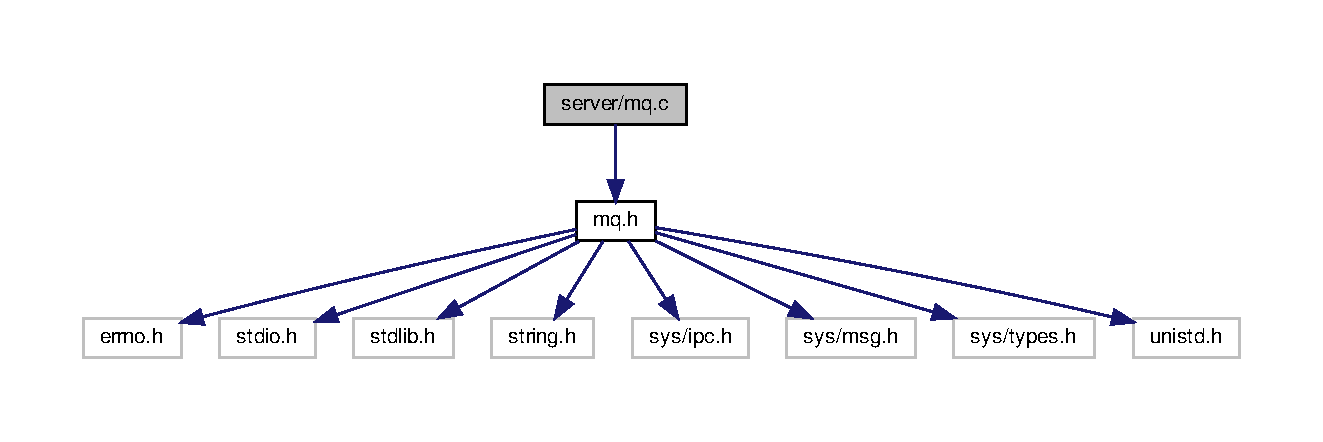
\includegraphics[width=350pt]{mq_8c__incl}
\end{center}
\end{figure}
\subsection*{Functions}
\begin{DoxyCompactItemize}
\item 
int \textbf{ mqid} ()
\begin{DoxyCompactList}\small\item\em Creation of the message queue id. \end{DoxyCompactList}\item 
char $\ast$ \textbf{ rcv\+\_\+msg} (int msqid, char $\ast$msg, long mtype)
\begin{DoxyCompactList}\small\item\em Wrapper to receive messages from the message queue. \end{DoxyCompactList}\item 
void \textbf{ snd\+\_\+msg} (int msqid, char $\ast$msg, long mtype)
\begin{DoxyCompactList}\small\item\em Wrapper to send messages to the message queue. \end{DoxyCompactList}\item 
void \textbf{ mq\+\_\+info} (int msqid)
\begin{DoxyCompactList}\small\item\em Get info from message queue. \end{DoxyCompactList}\end{DoxyCompactItemize}


\subsection{Function Documentation}
\mbox{\label{mq_8c_ad6373ac4d80e0c6198e95bb3a0515ff4}} 
\index{mq.\+c@{mq.\+c}!mq\+\_\+info@{mq\+\_\+info}}
\index{mq\+\_\+info@{mq\+\_\+info}!mq.\+c@{mq.\+c}}
\subsubsection{mq\+\_\+info()}
{\footnotesize\ttfamily void mq\+\_\+info (\begin{DoxyParamCaption}\item[{int}]{msqid }\end{DoxyParamCaption})}



Get info from message queue. 


\begin{DoxyParams}{Parameters}
{\em msqid} & \\
\hline
\end{DoxyParams}
\mbox{\label{mq_8c_aa6a2e92e60754c750bebd73bced350fd}} 
\index{mq.\+c@{mq.\+c}!mqid@{mqid}}
\index{mqid@{mqid}!mq.\+c@{mq.\+c}}
\subsubsection{mqid()}
{\footnotesize\ttfamily int mqid (\begin{DoxyParamCaption}\item[{void}]{ }\end{DoxyParamCaption})}



Creation of the message queue id. 

\begin{DoxyReturn}{Returns}
Message queue id 
\end{DoxyReturn}
\mbox{\label{mq_8c_a9fdea1732b3a3772bedad98f1a635e08}} 
\index{mq.\+c@{mq.\+c}!rcv\+\_\+msg@{rcv\+\_\+msg}}
\index{rcv\+\_\+msg@{rcv\+\_\+msg}!mq.\+c@{mq.\+c}}
\subsubsection{rcv\+\_\+msg()}
{\footnotesize\ttfamily char$\ast$ rcv\+\_\+msg (\begin{DoxyParamCaption}\item[{int}]{msqid,  }\item[{char $\ast$}]{msg,  }\item[{long}]{mtype }\end{DoxyParamCaption})}



Wrapper to receive messages from the message queue. 


\begin{DoxyParams}{Parameters}
{\em msqid} & Message queue ide \\
\hline
{\em msg} & Message received from message queue \\
\hline
{\em mtype} & Message type that identifies the process from which the message should be received \\
\hline
\end{DoxyParams}
\begin{DoxyReturn}{Returns}
String with the message extracted from the message queue 
\end{DoxyReturn}
\mbox{\label{mq_8c_a7d2e21e44f7a9a63f9f7a9020dd61719}} 
\index{mq.\+c@{mq.\+c}!snd\+\_\+msg@{snd\+\_\+msg}}
\index{snd\+\_\+msg@{snd\+\_\+msg}!mq.\+c@{mq.\+c}}
\subsubsection{snd\+\_\+msg()}
{\footnotesize\ttfamily void snd\+\_\+msg (\begin{DoxyParamCaption}\item[{int}]{msqid,  }\item[{char $\ast$}]{msg,  }\item[{long}]{mtype }\end{DoxyParamCaption})}



Wrapper to send messages to the message queue. 


\begin{DoxyParams}{Parameters}
{\em msqid} & Message queue ide \\
\hline
{\em msg} & Message received from message queue \\
\hline
{\em mtype} & Message type that identifies the process from which the message should be received \\
\hline
\end{DoxyParams}

\section{server/server.c File Reference}
\label{server_8c}\index{server/server.\+c@{server/server.\+c}}
{\ttfamily \#include \char`\"{}server.\+h\char`\"{}}\newline
Include dependency graph for server.\+c\+:
\nopagebreak
\begin{figure}[H]
\begin{center}
\leavevmode
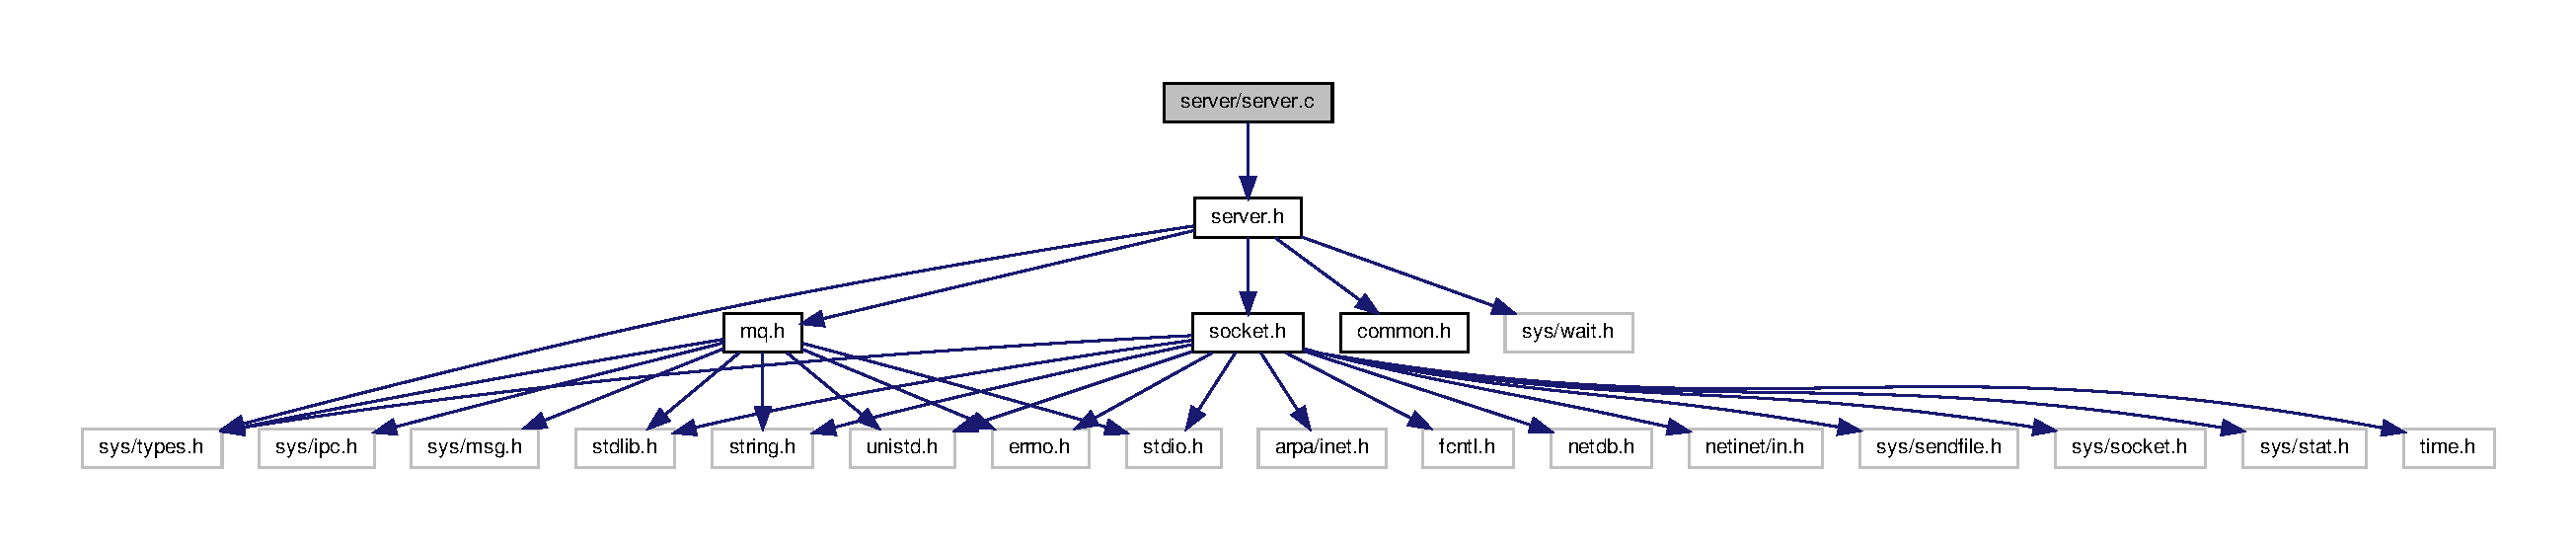
\includegraphics[width=350pt]{server_8c__incl}
\end{center}
\end{figure}
\subsection*{Functions}
\begin{DoxyCompactItemize}
\item 
int \textbf{ main} ()
\item 
void \textbf{ login\+\_\+handler} (int sockfd, int msqid)
\begin{DoxyCompactList}\small\item\em Login handler between auth and server. \end{DoxyCompactList}\item 
long \textbf{ get\+\_\+1st\+\_\+char} (char $\ast$str)
\begin{DoxyCompactList}\small\item\em Get the 1st char of str. \end{DoxyCompactList}\item 
long \textbf{ cmd\+\_\+handler} (char $\ast$cmd, char $\ast$msg)
\begin{DoxyCompactList}\small\item\em Decode the str that comes from the client and then be forwarded to A\+UT or F\+LS as appropriate. \end{DoxyCompactList}\item 
void \textbf{ rcv\+\_\+cmd} (int sockfd, int msqid)
\begin{DoxyCompactList}\small\item\em Login handler between [A\+UT] and [S\+RV]. \end{DoxyCompactList}\end{DoxyCompactItemize}


\subsection{Function Documentation}
\mbox{\label{server_8c_a9fab57195d50c5f2b55f2744232ad64d}} 
\index{server.\+c@{server.\+c}!cmd\+\_\+handler@{cmd\+\_\+handler}}
\index{cmd\+\_\+handler@{cmd\+\_\+handler}!server.\+c@{server.\+c}}
\subsubsection{cmd\+\_\+handler()}
{\footnotesize\ttfamily long cmd\+\_\+handler (\begin{DoxyParamCaption}\item[{char $\ast$}]{cmd,  }\item[{char $\ast$}]{msg }\end{DoxyParamCaption})}



Decode the str that comes from the client and then be forwarded to A\+UT or F\+LS as appropriate. 


\begin{DoxyParams}{Parameters}
{\em cmd} & \\
\hline
{\em msg} & \\
\hline
\end{DoxyParams}
\begin{DoxyReturn}{Returns}
long m\+\_\+type 
\end{DoxyReturn}
\mbox{\label{server_8c_a224345045f1250d5768d42d8cc9e3dab}} 
\index{server.\+c@{server.\+c}!get\+\_\+1st\+\_\+char@{get\+\_\+1st\+\_\+char}}
\index{get\+\_\+1st\+\_\+char@{get\+\_\+1st\+\_\+char}!server.\+c@{server.\+c}}
\subsubsection{get\+\_\+1st\+\_\+char()}
{\footnotesize\ttfamily long get\+\_\+1st\+\_\+char (\begin{DoxyParamCaption}\item[{char $\ast$}]{str }\end{DoxyParamCaption})}



Get the 1st char of str. 


\begin{DoxyParams}{Parameters}
{\em str} & \\
\hline
\end{DoxyParams}
\begin{DoxyReturn}{Returns}
long 
\end{DoxyReturn}
\mbox{\label{server_8c_a7c71d69d21fd5c82ce5af6aee230d25e}} 
\index{server.\+c@{server.\+c}!login\+\_\+handler@{login\+\_\+handler}}
\index{login\+\_\+handler@{login\+\_\+handler}!server.\+c@{server.\+c}}
\subsubsection{login\+\_\+handler()}
{\footnotesize\ttfamily void login\+\_\+handler (\begin{DoxyParamCaption}\item[{int}]{sockfd,  }\item[{int}]{msqid }\end{DoxyParamCaption})}



Login handler between auth and server. 


\begin{DoxyParams}{Parameters}
{\em sockfd} & \\
\hline
{\em msqid} & \\
\hline
\end{DoxyParams}
\mbox{\label{server_8c_ae66f6b31b5ad750f1fe042a706a4e3d4}} 
\index{server.\+c@{server.\+c}!main@{main}}
\index{main@{main}!server.\+c@{server.\+c}}
\subsubsection{main()}
{\footnotesize\ttfamily int main (\begin{DoxyParamCaption}\item[{void}]{ }\end{DoxyParamCaption})}

\mbox{\label{server_8c_abccdfc478d69333f46803552eba43cbb}} 
\index{server.\+c@{server.\+c}!rcv\+\_\+cmd@{rcv\+\_\+cmd}}
\index{rcv\+\_\+cmd@{rcv\+\_\+cmd}!server.\+c@{server.\+c}}
\subsubsection{rcv\+\_\+cmd()}
{\footnotesize\ttfamily void rcv\+\_\+cmd (\begin{DoxyParamCaption}\item[{int}]{sockfd,  }\item[{int}]{msqid }\end{DoxyParamCaption})}



Login handler between [A\+UT] and [S\+RV]. 


\begin{DoxyParams}{Parameters}
{\em sockfd} & \\
\hline
{\em msqid} & \\
\hline
\end{DoxyParams}

\section{server/socket\+\_\+server.c File Reference}
\label{socket__server_8c}\index{server/socket\+\_\+server.\+c@{server/socket\+\_\+server.\+c}}
{\ttfamily \#include \char`\"{}socket.\+h\char`\"{}}\newline
Include dependency graph for socket\+\_\+server.\+c\+:\nopagebreak
\begin{figure}[H]
\begin{center}
\leavevmode
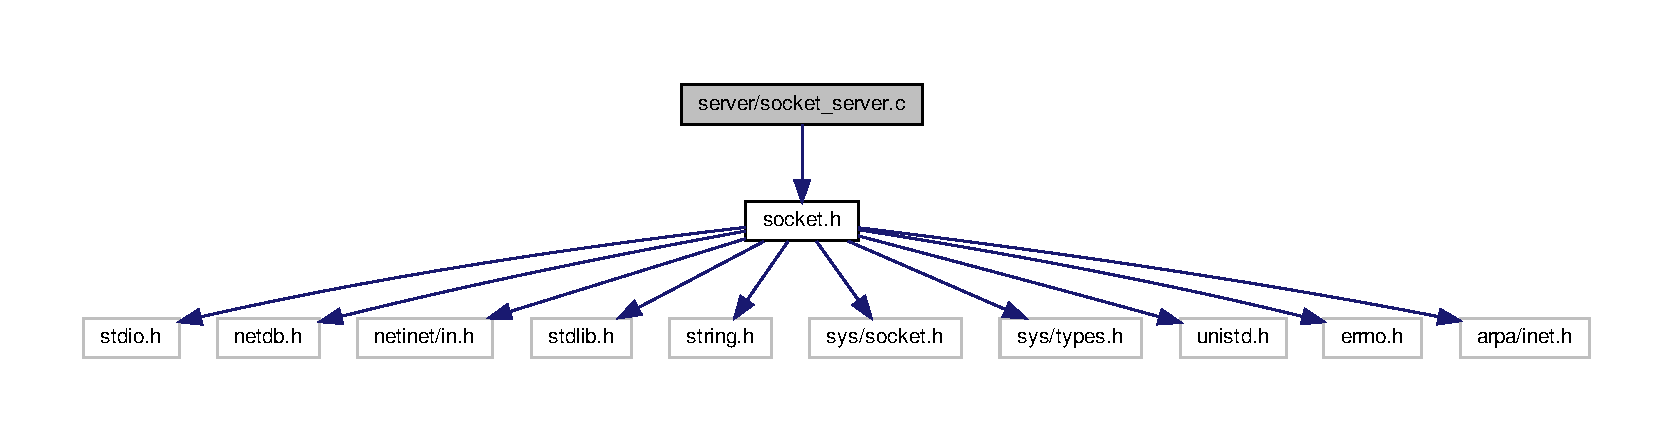
\includegraphics[width=350pt]{socket__server_8c__incl}
\end{center}
\end{figure}
\subsection*{Functions}
\begin{DoxyCompactItemize}
\item 
int \textbf{ srv\+\_\+socket} ()
\begin{DoxyCompactList}\small\item\em Create, assign port, bind and listen of socket server. \end{DoxyCompactList}\end{DoxyCompactItemize}


\subsection{Function Documentation}
\mbox{\label{socket__server_8c_abaa85d7aff16c338adf9a408c151bc28}} 
\index{socket\+\_\+server.\+c@{socket\+\_\+server.\+c}!srv\+\_\+socket@{srv\+\_\+socket}}
\index{srv\+\_\+socket@{srv\+\_\+socket}!socket\+\_\+server.\+c@{socket\+\_\+server.\+c}}
\subsubsection{srv\+\_\+socket()}
{\footnotesize\ttfamily int srv\+\_\+socket (\begin{DoxyParamCaption}{ }\end{DoxyParamCaption})}



Create, assign port, bind and listen of socket server. 

\begin{DoxyReturn}{Returns}
int sockfd 
\end{DoxyReturn}

\input{burn_8c}
\input{example_8c}
\section{thrash/file.c File Reference}
\label{file_8c}\index{thrash/file.\+c@{thrash/file.\+c}}
{\ttfamily \#include \char`\"{}auth.\+h\char`\"{}}\newline
{\ttfamily \#include \char`\"{}mq.\+h\char`\"{}}\newline
{\ttfamily \#include $<$sys/types.\+h$>$}\newline
{\ttfamily \#include $<$sys/wait.\+h$>$}\newline
Include dependency graph for file.\+c\+:\nopagebreak
\begin{figure}[H]
\begin{center}
\leavevmode
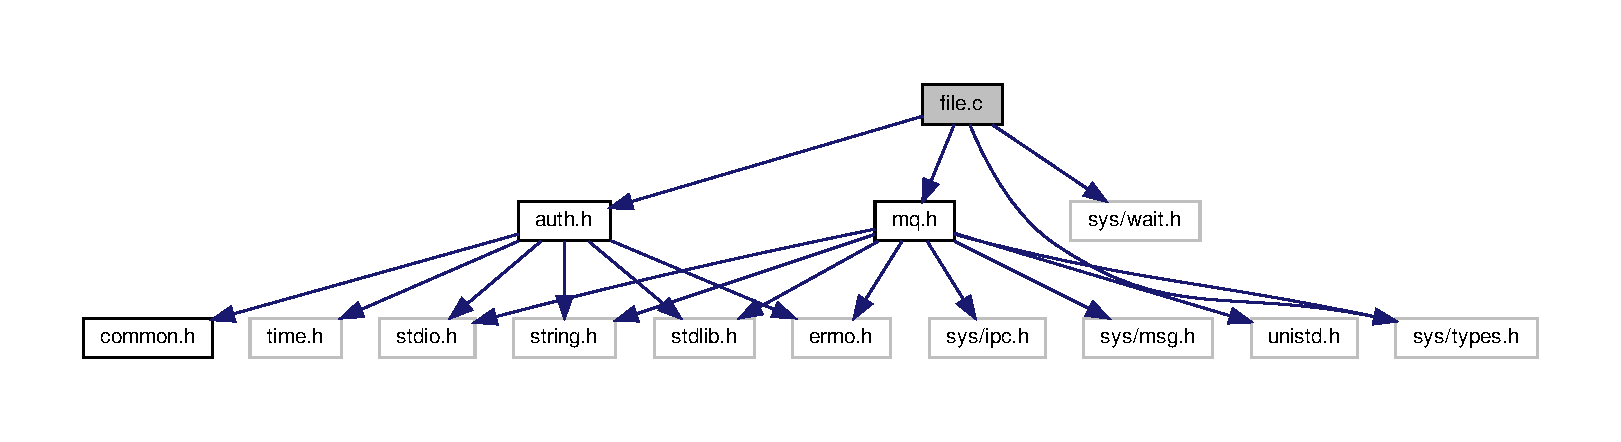
\includegraphics[width=350pt]{file_8c__incl}
\end{center}
\end{figure}
\subsection*{Functions}
\begin{DoxyCompactItemize}
\item 
int \textbf{ cmd\+\_\+handler} (int msqid)
\begin{DoxyCompactList}\small\item\em Login handler between auth and srv. \end{DoxyCompactList}\item 
int \textbf{ main} (void)
\end{DoxyCompactItemize}


\subsection{Function Documentation}
\mbox{\label{file_8c_a975d9337db509c0204b110f51d723160}} 
\index{file.\+c@{file.\+c}!cmd\+\_\+handler@{cmd\+\_\+handler}}
\index{cmd\+\_\+handler@{cmd\+\_\+handler}!file.\+c@{file.\+c}}
\subsubsection{cmd\+\_\+handler()}
{\footnotesize\ttfamily int cmd\+\_\+handler (\begin{DoxyParamCaption}\item[{int}]{msqid }\end{DoxyParamCaption})}



Login handler between auth and srv. 

Command handler.


\begin{DoxyParams}{Parameters}
{\em msqid} & \\
\hline
\end{DoxyParams}
\mbox{\label{file_8c_a840291bc02cba5474a4cb46a9b9566fe}} 
\index{file.\+c@{file.\+c}!main@{main}}
\index{main@{main}!file.\+c@{file.\+c}}
\subsubsection{main()}
{\footnotesize\ttfamily int main (\begin{DoxyParamCaption}\item[{void}]{ }\end{DoxyParamCaption})}


\section{thrash/main.c File Reference}
\label{main_8c}\index{thrash/main.\+c@{thrash/main.\+c}}
\subsection*{Functions}
\begin{DoxyCompactItemize}
\item 
char $\ast$ \textbf{ readable\+\_\+fs} (long int size, char $\ast$buf)
\begin{DoxyCompactList}\small\item\em Parser that returns in human-\/readable format the size of a file. \end{DoxyCompactList}\item 
int \textbf{ main} ()
\end{DoxyCompactItemize}


\subsection{Function Documentation}
\mbox{\label{main_8c_ae66f6b31b5ad750f1fe042a706a4e3d4}} 
\index{main.\+c@{main.\+c}!main@{main}}
\index{main@{main}!main.\+c@{main.\+c}}
\subsubsection{main()}
{\footnotesize\ttfamily int main (\begin{DoxyParamCaption}\item[{void}]{ }\end{DoxyParamCaption})}

\mbox{\label{main_8c_acb8985a720cf17b68e99872ba793f2cc}} 
\index{main.\+c@{main.\+c}!readable\+\_\+fs@{readable\+\_\+fs}}
\index{readable\+\_\+fs@{readable\+\_\+fs}!main.\+c@{main.\+c}}
\subsubsection{readable\+\_\+fs()}
{\footnotesize\ttfamily char$\ast$ readable\+\_\+fs (\begin{DoxyParamCaption}\item[{long int}]{size,  }\item[{char $\ast$}]{buf }\end{DoxyParamCaption})}



Parser that returns in human-\/readable format the size of a file. 


\begin{DoxyParams}{Parameters}
{\em size} & in bytes from file \\
\hline
{\em buf} & string \\
\hline
\end{DoxyParams}
\begin{DoxyReturn}{Returns}
Formatted string what contains human-\/readable size of file 
\end{DoxyReturn}

\section{prueba.\+c File Reference}
\label{prueba_8c}\index{prueba.\+c@{prueba.\+c}}
{\ttfamily \#include $<$stdlib.\+h$>$}\newline
{\ttfamily \#include $<$stdio.\+h$>$}\newline
{\ttfamily \#include $<$string.\+h$>$}\newline
Include dependency graph for prueba.\+c\+:\nopagebreak
\begin{figure}[H]
\begin{center}
\leavevmode
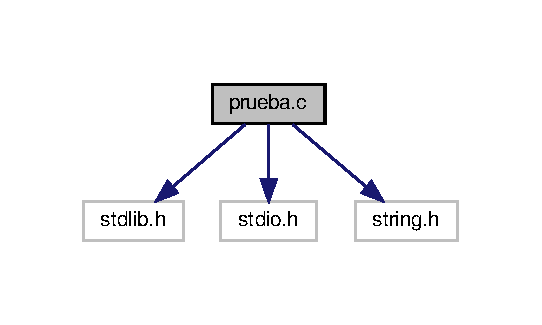
\includegraphics[width=260pt]{prueba_8c__incl}
\end{center}
\end{figure}
\subsection*{Macros}
\begin{DoxyCompactItemize}
\item 
\#define \textbf{ B\+U\+F\+F\+S\+I\+ZE}~256
\end{DoxyCompactItemize}
\subsection*{Functions}
\begin{DoxyCompactItemize}
\item 
long \textbf{ get\+\_\+1st\+\_\+char} (char $\ast$str)
\item 
long \textbf{ cmd\+\_\+handler} (char $\ast$cmd, char $\ast$msg)
\item 
int \textbf{ main} ()
\end{DoxyCompactItemize}


\subsection{Macro Definition Documentation}
\mbox{\label{prueba_8c_a39912bfe2a55f30e269196f9141d845d}} 
\index{prueba.\+c@{prueba.\+c}!B\+U\+F\+F\+S\+I\+ZE@{B\+U\+F\+F\+S\+I\+ZE}}
\index{B\+U\+F\+F\+S\+I\+ZE@{B\+U\+F\+F\+S\+I\+ZE}!prueba.\+c@{prueba.\+c}}
\subsubsection{B\+U\+F\+F\+S\+I\+ZE}
{\footnotesize\ttfamily \#define B\+U\+F\+F\+S\+I\+ZE~256}



\subsection{Function Documentation}
\mbox{\label{prueba_8c_a9fab57195d50c5f2b55f2744232ad64d}} 
\index{prueba.\+c@{prueba.\+c}!cmd\+\_\+handler@{cmd\+\_\+handler}}
\index{cmd\+\_\+handler@{cmd\+\_\+handler}!prueba.\+c@{prueba.\+c}}
\subsubsection{cmd\+\_\+handler()}
{\footnotesize\ttfamily long cmd\+\_\+handler (\begin{DoxyParamCaption}\item[{char $\ast$}]{cmd,  }\item[{char $\ast$}]{msg }\end{DoxyParamCaption})}

\mbox{\label{prueba_8c_a224345045f1250d5768d42d8cc9e3dab}} 
\index{prueba.\+c@{prueba.\+c}!get\+\_\+1st\+\_\+char@{get\+\_\+1st\+\_\+char}}
\index{get\+\_\+1st\+\_\+char@{get\+\_\+1st\+\_\+char}!prueba.\+c@{prueba.\+c}}
\subsubsection{get\+\_\+1st\+\_\+char()}
{\footnotesize\ttfamily long get\+\_\+1st\+\_\+char (\begin{DoxyParamCaption}\item[{char $\ast$}]{str }\end{DoxyParamCaption})}

\mbox{\label{prueba_8c_ae66f6b31b5ad750f1fe042a706a4e3d4}} 
\index{prueba.\+c@{prueba.\+c}!main@{main}}
\index{main@{main}!prueba.\+c@{prueba.\+c}}
\subsubsection{main()}
{\footnotesize\ttfamily int main (\begin{DoxyParamCaption}\item[{void}]{ }\end{DoxyParamCaption})}


\section{thrash/receiver2.c File Reference}
\label{receiver2_8c}\index{thrash/receiver2.\+c@{thrash/receiver2.\+c}}
{\ttfamily \#include $<$stdio.\+h$>$}\newline
{\ttfamily \#include $<$sys/ipc.\+h$>$}\newline
{\ttfamily \#include $<$sys/msg.\+h$>$}\newline
{\ttfamily \#include \char`\"{}mq.\+h\char`\"{}}\newline
Include dependency graph for receiver2.\+c\+:\nopagebreak
\begin{figure}[H]
\begin{center}
\leavevmode
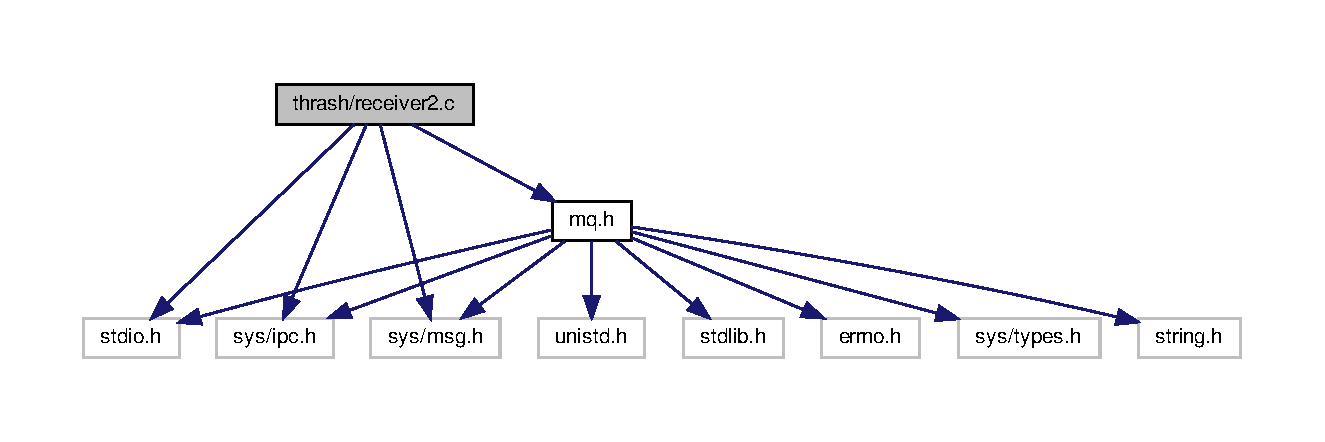
\includegraphics[width=350pt]{receiver2_8c__incl}
\end{center}
\end{figure}
\subsection*{Functions}
\begin{DoxyCompactItemize}
\item 
int \textbf{ main} ()
\end{DoxyCompactItemize}


\subsection{Function Documentation}
\mbox{\label{receiver2_8c_ae66f6b31b5ad750f1fe042a706a4e3d4}} 
\index{receiver2.\+c@{receiver2.\+c}!main@{main}}
\index{main@{main}!receiver2.\+c@{receiver2.\+c}}
\subsubsection{main()}
{\footnotesize\ttfamily int main (\begin{DoxyParamCaption}\item[{void}]{ }\end{DoxyParamCaption})}


\input{recfile_8c}
\section{thrash/sender2.c File Reference}
\label{sender2_8c}\index{thrash/sender2.\+c@{thrash/sender2.\+c}}
{\ttfamily \#include $<$stdio.\+h$>$}\newline
{\ttfamily \#include $<$sys/ipc.\+h$>$}\newline
{\ttfamily \#include $<$sys/msg.\+h$>$}\newline
{\ttfamily \#include \char`\"{}mq.\+h\char`\"{}}\newline
Include dependency graph for sender2.\+c\+:
\nopagebreak
\begin{figure}[H]
\begin{center}
\leavevmode
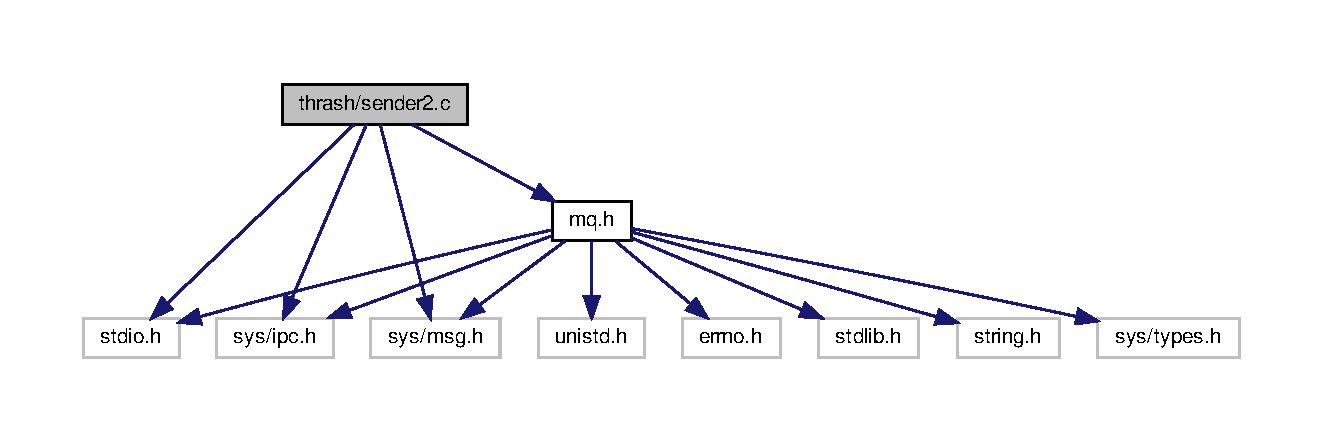
\includegraphics[width=350pt]{sender2_8c__incl}
\end{center}
\end{figure}
\subsection*{Functions}
\begin{DoxyCompactItemize}
\item 
int \textbf{ main} ()
\end{DoxyCompactItemize}


\subsection{Function Documentation}
\mbox{\label{sender2_8c_ae66f6b31b5ad750f1fe042a706a4e3d4}} 
\index{sender2.\+c@{sender2.\+c}!main@{main}}
\index{main@{main}!sender2.\+c@{sender2.\+c}}
\subsubsection{main()}
{\footnotesize\ttfamily int main (\begin{DoxyParamCaption}\item[{void}]{ }\end{DoxyParamCaption})}


\input{sendfile_8c}
\section{signal.\+c File Reference}
\label{signal_8c}\index{signal.\+c@{signal.\+c}}
{\ttfamily \#include $<$stdio.\+h$>$}\newline
{\ttfamily \#include $<$signal.\+h$>$}\newline
{\ttfamily \#include $<$stdlib.\+h$>$}\newline
{\ttfamily \#include $<$unistd.\+h$>$}\newline
Include dependency graph for signal.\+c\+:\nopagebreak
\begin{figure}[H]
\begin{center}
\leavevmode
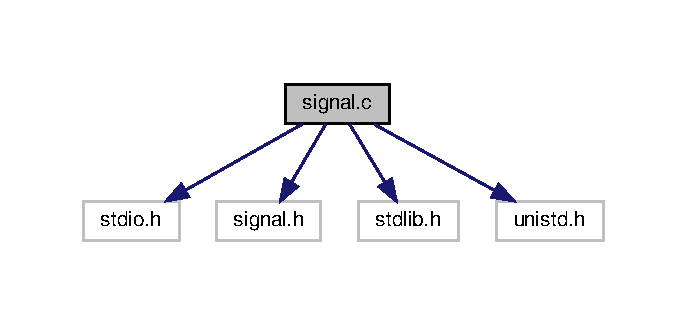
\includegraphics[width=330pt]{signal_8c__incl}
\end{center}
\end{figure}
\subsection*{Functions}
\begin{DoxyCompactItemize}
\item 
void \textbf{ sig\+\_\+handler} (int signo)
\item 
int \textbf{ main} (void)
\item 
void \textbf{ I\+N\+Thandler} (int sig)
\end{DoxyCompactItemize}


\subsection{Function Documentation}
\mbox{\label{signal_8c_a6a3869251603ae4e569abadbd7dab11c}} 
\index{signal.\+c@{signal.\+c}!I\+N\+Thandler@{I\+N\+Thandler}}
\index{I\+N\+Thandler@{I\+N\+Thandler}!signal.\+c@{signal.\+c}}
\subsubsection{I\+N\+Thandler()}
{\footnotesize\ttfamily void I\+N\+Thandler (\begin{DoxyParamCaption}\item[{int}]{sig }\end{DoxyParamCaption})}

\mbox{\label{signal_8c_a840291bc02cba5474a4cb46a9b9566fe}} 
\index{signal.\+c@{signal.\+c}!main@{main}}
\index{main@{main}!signal.\+c@{signal.\+c}}
\subsubsection{main()}
{\footnotesize\ttfamily int main (\begin{DoxyParamCaption}\item[{void}]{ }\end{DoxyParamCaption})}

\mbox{\label{signal_8c_a4f31a6fd48ee5d4579ae4aaaa3cae285}} 
\index{signal.\+c@{signal.\+c}!sig\+\_\+handler@{sig\+\_\+handler}}
\index{sig\+\_\+handler@{sig\+\_\+handler}!signal.\+c@{signal.\+c}}
\subsubsection{sig\+\_\+handler()}
{\footnotesize\ttfamily void sig\+\_\+handler (\begin{DoxyParamCaption}\item[{int}]{signo }\end{DoxyParamCaption})}


\section{thrash/socket.c File Reference}
\label{socket_8c}\index{thrash/socket.\+c@{thrash/socket.\+c}}
{\ttfamily \#include \char`\"{}socket.\+h\char`\"{}}\newline
Include dependency graph for socket.\+c\+:\nopagebreak
\begin{figure}[H]
\begin{center}
\leavevmode
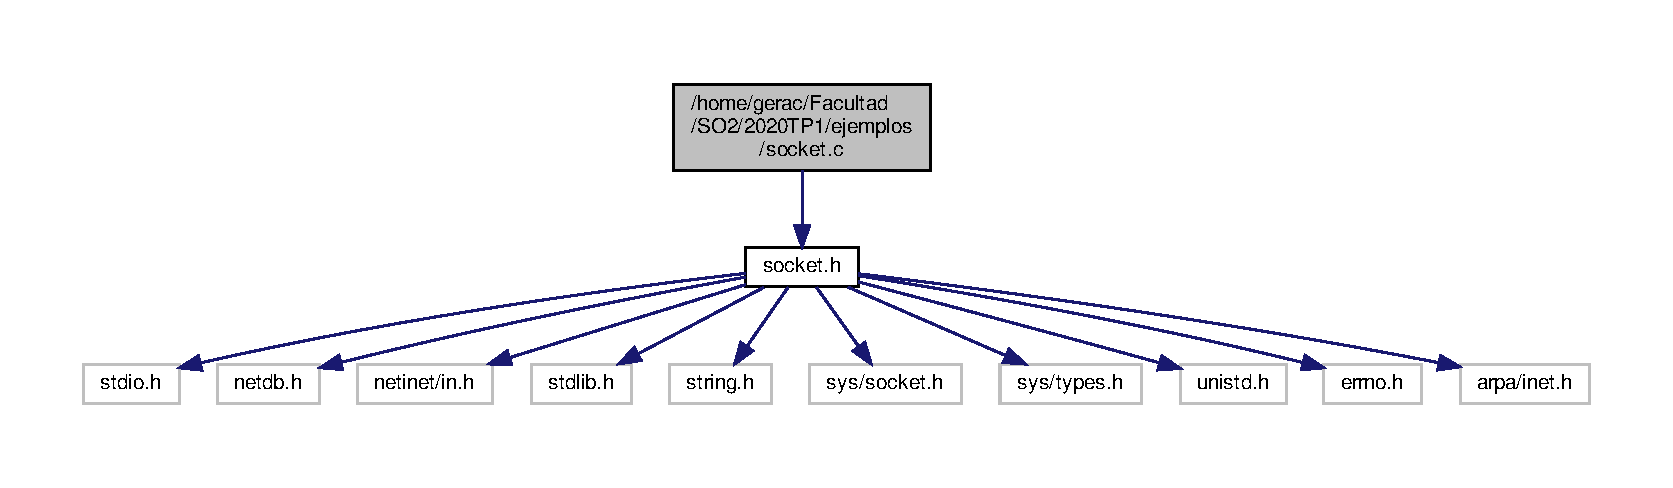
\includegraphics[width=350pt]{socket_8c__incl}
\end{center}
\end{figure}
\subsection*{Functions}
\begin{DoxyCompactItemize}
\item 
int \textbf{ srv\+\_\+socket} ()
\begin{DoxyCompactList}\small\item\em Create, assign port, bind and listen of socket server. \end{DoxyCompactList}\item 
int \textbf{ wait\+\_\+cli} (int sockfd)
\begin{DoxyCompactList}\small\item\em Waiting for the client to connect. \end{DoxyCompactList}\item 
int \textbf{ cli\+\_\+socket} ()
\begin{DoxyCompactList}\small\item\em Creation, assign IP and port of client socket. Connect to server is included. \end{DoxyCompactList}\item 
void \textbf{ send\+\_\+file} (int connfd, char $\ast$filename)
\begin{DoxyCompactList}\small\item\em Send the file through sendfile function that maximizes the transfer speed using zero copy. \end{DoxyCompactList}\item 
void \textbf{ recv\+\_\+file} (int newsockfd)
\begin{DoxyCompactList}\small\item\em Función para recibir archivos vía T\+CP. \end{DoxyCompactList}\end{DoxyCompactItemize}


\subsection{Function Documentation}
\mbox{\label{socket_8c_a9c129efbce40f3061d7899d2adf36a55}} 
\index{socket.\+c@{socket.\+c}!cli\+\_\+socket@{cli\+\_\+socket}}
\index{cli\+\_\+socket@{cli\+\_\+socket}!socket.\+c@{socket.\+c}}
\subsubsection{cli\+\_\+socket()}
{\footnotesize\ttfamily int cli\+\_\+socket (\begin{DoxyParamCaption}\item[{void}]{ }\end{DoxyParamCaption})}



Creation, assign IP and port of client socket. Connect to server is included. 

\begin{DoxyReturn}{Returns}
sockfd 
\end{DoxyReturn}
\mbox{\label{socket_8c_afe49ab8d5d6dbc407156f33dce0152cf}} 
\index{socket.\+c@{socket.\+c}!recv\+\_\+file@{recv\+\_\+file}}
\index{recv\+\_\+file@{recv\+\_\+file}!socket.\+c@{socket.\+c}}
\subsubsection{recv\+\_\+file()}
{\footnotesize\ttfamily void recv\+\_\+file (\begin{DoxyParamCaption}\item[{int}]{newsockfd }\end{DoxyParamCaption})}



Función para recibir archivos vía T\+CP. 


\begin{DoxyParams}{Parameters}
{\em newsockfd} & \\
\hline
{\em nombre\+Archivo} & \\
\hline
\end{DoxyParams}
\mbox{\label{socket_8c_a91bd21665371000f5251a149716f82fb}} 
\index{socket.\+c@{socket.\+c}!send\+\_\+file@{send\+\_\+file}}
\index{send\+\_\+file@{send\+\_\+file}!socket.\+c@{socket.\+c}}
\subsubsection{send\+\_\+file()}
{\footnotesize\ttfamily void send\+\_\+file (\begin{DoxyParamCaption}\item[{int}]{connfd,  }\item[{char $\ast$}]{filename }\end{DoxyParamCaption})}



Send the file through sendfile function that maximizes the transfer speed using zero copy. 


\begin{DoxyParams}{Parameters}
{\em connfd} & socket file descriptor \\
\hline
{\em str} & file without folder path \\
\hline
\end{DoxyParams}
\mbox{\label{socket_8c_abaa85d7aff16c338adf9a408c151bc28}} 
\index{socket.\+c@{socket.\+c}!srv\+\_\+socket@{srv\+\_\+socket}}
\index{srv\+\_\+socket@{srv\+\_\+socket}!socket.\+c@{socket.\+c}}
\subsubsection{srv\+\_\+socket()}
{\footnotesize\ttfamily int srv\+\_\+socket (\begin{DoxyParamCaption}\item[{void}]{ }\end{DoxyParamCaption})}



Create, assign port, bind and listen of socket server. 

\begin{DoxyReturn}{Returns}
int sockfd 
\end{DoxyReturn}
\mbox{\label{socket_8c_ad26b08974642b47dc5bf48289824f655}} 
\index{socket.\+c@{socket.\+c}!wait\+\_\+cli@{wait\+\_\+cli}}
\index{wait\+\_\+cli@{wait\+\_\+cli}!socket.\+c@{socket.\+c}}
\subsubsection{wait\+\_\+cli()}
{\footnotesize\ttfamily int wait\+\_\+cli (\begin{DoxyParamCaption}\item[{int}]{sockfd }\end{DoxyParamCaption})}



Waiting for the client to connect. 


\begin{DoxyParams}{Parameters}
{\em sockfd} & \\
\hline
\end{DoxyParams}
\begin{DoxyReturn}{Returns}
int sockfd 
\end{DoxyReturn}

\section{test.\+c File Reference}
\label{test_8c}\index{test.\+c@{test.\+c}}
{\ttfamily \#include $<$sys/types.\+h$>$}\newline
{\ttfamily \#include $<$sys/ipc.\+h$>$}\newline
{\ttfamily \#include $<$sys/msg.\+h$>$}\newline
{\ttfamily \#include $<$stdio.\+h$>$}\newline
{\ttfamily \#include $<$errno.\+h$>$}\newline
Include dependency graph for test.\+c\+:\nopagebreak
\begin{figure}[H]
\begin{center}
\leavevmode
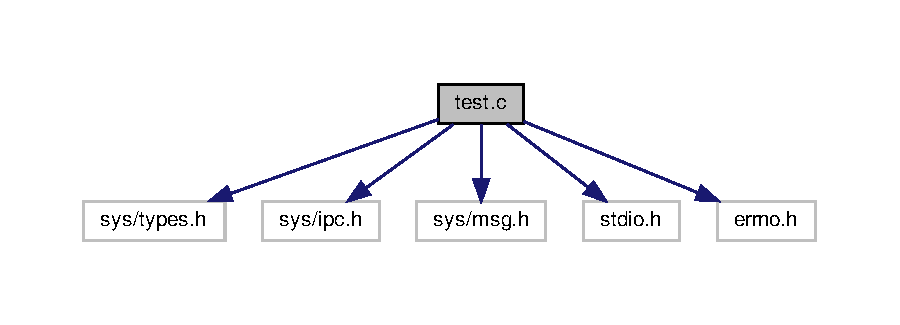
\includegraphics[width=350pt]{test_8c__incl}
\end{center}
\end{figure}
\subsection*{Data Structures}
\begin{DoxyCompactItemize}
\item 
struct \textbf{ msgbuf}
\end{DoxyCompactItemize}
\subsection*{Functions}
\begin{DoxyCompactItemize}
\item 
int \textbf{ main} (void)
\end{DoxyCompactItemize}


\subsection{Function Documentation}
\mbox{\label{test_8c_a840291bc02cba5474a4cb46a9b9566fe}} 
\index{test.\+c@{test.\+c}!main@{main}}
\index{main@{main}!test.\+c@{test.\+c}}
\subsubsection{main()}
{\footnotesize\ttfamily int main (\begin{DoxyParamCaption}\item[{void}]{ }\end{DoxyParamCaption})}


%--- End generated contents ---

% Index
\backmatter
\newpage
\phantomsection
\clearemptydoublepage
\addcontentsline{toc}{chapter}{Index}
\printindex

\end{document}
